\documentclass[a4,center,fleqn]{NAR}

%\usepackage{NAR-natbib}
\usepackage{graphics}
%\usepackage[latin1]{inputenc}
\usepackage{subcaption}
\usepackage{verbatim}%for comments
\usepackage[table,x11names,dvipsnames]{xcolor}
\usepackage{adjustbox}% to resize figures
%\usepackage[skip=4pt]{caption}  % to keep dstance between caption and table/figure
%\usepackage[sort&compress]{natbib}
\usepackage{xspace}
%\usepackage{algorithm}
%\usepackage{algpseudocode}
\usepackage{amsmath}
\usepackage{xcolor}
\usepackage{todonotes}
\usepackage{booktabs}
\usepackage{relsize}
\usepackage{lipsum}
\usepackage{collcell}
\usepackage{pgfkeys}
\usepackage{amsmath}
\usepackage{varwidth}
\usepackage{tikz}
\usepackage{makecell}
\usepackage{gensymb}
\usepackage{inconsolata}

%%%%%% TIKZ %%%%%%%%%%%%%%%%%%%%%%%%


\usetikzlibrary{shapes.geometric, arrows,calc,fit,positioning}



\usetikzlibrary{shapes.geometric, arrows,calc}
%\tikzset { *|/.style={to path={	(perpendicular cs : horizontal line through ={(\tikztostart)},	vertical line through{(\tikztotarget)})	--(\tikztotarget) \tikztonodes	}	}	}

\pgfdeclarelayer{background}
\pgfdeclarelayer{foreground}
\pgfsetlayers{background,main,foreground}

\tikzstyle{startend}=[rectangle, rounded corners, minimum width=2cm,  minimum height=1cm, text width =2cm, text centered, draw=none, fill= orange!50, font=\sf]
\tikzstyle{io}=[trapezium, trapezium left angle=70,trapezium right angle= 110,minimum width=3.9cm, minimum height=1cm, text centered, draw=none, fill= blue!30, font=\sf]

\tikzstyle{process}=[rectangle, minimum width=3cm,maximum width=3, minimum height=1cm, text centered, draw=black, fill= orange!30, font=\sffamily]
\tikzstyle{Vprocess}=[rectangle, minimum width=6cm, minimum height=1cm, text centered, font=\sf\bfseries,  fill= gray!80, draw=none, text=white]
\tikzstyle{VSprocess}=[rectangle, minimum width=1cm, minimum height=2cm, text centered, font=\sf\bfseries,  fill= gray!80, draw=none, text=white]
\tikzstyle{squareprocess}=[rectangle, minimum width=2cm, minimum height=7cm, text centered, draw=black, fill= orange!30, font=\sffamily]
\tikzstyle{Bprocess}=[rectangle, minimum width=6cm, minimum height=1cm, text centered,  font=\sf\bfseries,  fill= cyan!60!black, draw=none, text=white]
\tikzstyle{BSprocess}=[rectangle, minimum width=3cm, minimum height=1cm, text centered, draw=black, fill= orange!30, font=\sffamily]
\tikzstyle{decision}=[diamond, minimum width=2.5cm, minimum height=1.5cm, align=center, inner sep=-5pt ,font=\sf\bfseries,  fill= PineGreen!60, draw=none, text=white]
\tikzstyle{IO}=[text=white]

\tikzstyle{arrow}=[line width=1.5pt, ->, >=stealth, gray!80!black]
\tikzstyle{arrowcaption}=[font=\sf\relsize{+1},black]
\tikzstyle{input}=[fill= gray!80!black, inner sep=5pt,rounded corners=5pt]
\tikzstyle{output}=[fill= gray!80!black, inner sep=5pt,rounded corners=5pt]

\pgfkeys{/heat/.is family, /heat,
	Max colour/.initial = Green4,
	Min colour/.initial = Red1,
	max colour/.initial = SpringGreen3,
	mid colour/.initial = white,
	min colour/.initial = Yellow1,
	text colour/.initial = black,
	Min color/.style = {Min colour=#1},% for our friends who can't spell
	Max color/.style = {Max colour=#1},
	min color/.style = {min colour=#1},
	mid color/.style = {mid colour=#1},
	max color/.style = {max colour=#1},
	text color/.style = {text colour=#1},
	min/.initial = -1,
	mid/.initial = 0,
	max/.initial = 1,
	slider/.code={%
		\tikz{\shade[left color=\HVal{min colour},%
			right color=\HVal{max colour}]%
			(current page.south west) rectangle ++(#1,12pt);
		}%
	}%
}

\newcommand{\tikzcircle}[2][red,fill=red]{\tikz[baseline=-0.5ex]\draw[#1,radius=#2] (0,0) circle ;}%
\newcommand\Heatset[1]{\pgfkeys{/heat, #1}}
\newcommand\HVal[1]{\pgfkeysvalueof{/heat/#1}}

\newcolumntype{H}{>{\collectcell\Heat}r<{\endcollectcell}}
\newcommand\Heat[1]{% \Heat{number in the interval [min, max] }
	\if\relax\detokenize{#1}\relax% empty cell
	\else%
	\pgfmathparse{int(100*(#1-\HVal{min})/(\HVal{max}-\HVal{min}))}% map number to [0,100]
	\ifnum\pgfmathresult>100% too big
	\edef\HeatCell{\noexpand\cellcolor{\HVal{Max colour}}}%
	\else\ifnum\pgfmathresult<0% too small
	\edef\HeatCell{\noexpand\cellcolor{\HVal{Min colour}}}%
	\else\ifnum\pgfmathresult<50% between min and mid
	\pgfmathparse{int(2*\pgfmathresult)}% map number to [0,100]
	\edef\HeatCell{\noexpand\cellcolor{\HVal{mid colour}!\pgfmathresult!\HVal{min colour}}}%
	\else% between min and max
	\pgfmathparse{int(2*(\pgfmathresult-50))}% map number to [0,100]
	\edef\HeatCell{\noexpand\cellcolor{\HVal{max colour}!\pgfmathresult!\HVal{mid colour}}}%
	\fi%
	\fi%
	\fi%
	\HeatCell\textcolor{\HVal{text colour}}{$#1$}%
	\fi%
}

\pgfkeys{/heatsec/.is family, /heatsec,
	Max colour/.initial = Green4,
	Min colour/.initial = Red1,
	max colour/.initial = SpringGreen3,
	mid colour/.initial = white,
	min colour/.initial = Yellow1,
	text colour/.initial = black,
	Min color/.style = {Min colour=#1},% for our friends who can't spell
	Max color/.style = {Max colour=#1},
	min color/.style = {min colour=#1},
	mid color/.style = {mid colour=#1},
	max color/.style = {max colour=#1},
	text color/.style = {text colour=#1},
	min/.initial = -1,
	mid/.initial = 0,
	max/.initial = 1,
	slider/.code={%
		\tikz{\shade[left color=\HVal{min colour},%
			right color=\HVal{max colour}]%
			(current page.south west) rectangle ++(#1,12pt);
		}%
	}%
}
\newcommand\HeatSecset[1]{\pgfkeys{/heatsec, #1}}
\newcommand\HSVal[1]{\pgfkeysvalueof{/heatsec/#1}}

\colorlet{BadCol}{Burlywood1!70!red}


\newcolumntype{S}{>{\collectcell\HeatSec}r<{\endcollectcell}}
\newcommand\HeatSec[1]{% \Heat{number in the interval [min, max] }
	\if\relax\detokenize{#1}\relax% empty cell
	\else%
	\pgfmathparse{int(100*(#1-\HSVal{min})/(\HSVal{max}-\HSVal{min}))}% map number to [0,100]
	\ifnum\pgfmathresult>100% too big
	\edef\HeatCell{\noexpand\cellcolor{\HSVal{Max colour}}}%
	\else\ifnum\pgfmathresult<0% too small
	\edef\HeatCell{\noexpand\cellcolor{\HSVal{Min colour}}}%
	\else\ifnum\pgfmathresult<50% between min and mid
	\pgfmathparse{int(2*\pgfmathresult)}% map number to [0,100]
	\edef\HeatCell{\noexpand\cellcolor{\HSVal{mid colour}!\pgfmathresult!\HSVal{min colour}}}%
	\else% between min and max
	\pgfmathparse{int(2*(\pgfmathresult-50))}% map number to [0,100]
	\edef\HeatCell{\noexpand\cellcolor{\HSVal{max colour}!\pgfmathresult!\HSVal{mid colour}}}%
	\fi%
	\fi%
	\fi%
	\HeatCell\textcolor{\HSVal{text colour}}{$#1$}%
	\fi%
}

%%%%%% MACROS %%%%%%%%%%%%%%%%%%%%%%%%

\definecolor{lightsalmon}{rgb}{1.0, 0.63, 0.48}
\definecolor{lightseagreen}{rgb}{0.13, 0.7, 0.67}
\definecolor{americanrose}{rgb}{1.0, 0.01, 0.24}
\DeclareMathOperator*{\argmin}{\arg\!\min}
\DeclareMathOperator*{\argmax}{\arg\!\max}
\newcommand{\multicoomment}[1]{}
\newcommand{\Software}[1]{\text{\ttfamily\bfseries #1}}
\newcommand{\OurTool}{\Software{IPANEMAP}\xspace}
\newcommand{\SM }{{\tt SHAPEMap}\xspace}
\newcommand{\SH }{{\tt SHAPE}\xspace}
\newcommand{\VP }{{\tt Vienna package}\xspace}
\newcommand{\OurRna}{\Software{Did}\xspace}
\newcommand{\mm }{{\tt$M\&M$}\xspace}
\newcommand{\DP }{{\tt DP}\xspace}
\newcommand{\didy }{{\sf GIR1 Lariat-capping ribozyme}\xspace}

\newcommand{\CE }{{\tt capillary electrophoresis}\xspace}
%MPCRnas MultiProbing Conformers}}
% Macros for # variables
\newcommand{\BP }{{\mathcal{ BP}}}
\newcommand{\Ensemble }{{\mathcal{ S}}}
\newcommand{\Sample }{{\mathcal{ S_D}}}
\newcommand{\PData }[1]{{\mathcal{ D}_{#1}}}
\newcommand{\Bzcond}[1]{ \mathbb{P}(s\mid #1)}
\newcommand{\CBP}[1]{ \mathbb{CP}_#1}
\newcommand{\BF}{ \mathbb{BF}}
\newcommand{\Zed}{\mathbb{Z}}
\newcommand{\Edist }{{ \text{Dist}}}
\newcommand{\RL }{{n}}
\newcommand{\CL}{MBkM\xspace}
\newcommand{\Clusters}{\mathcal{C}}
\newcommand{\Centroids}{\mathcal{C_O}}
\newcommand{\GMean}{\text{GM}}
\newcommand{\Ref}{R}
%\newcommand{\OurRna}{\Software{Did}}
%MPCRnas MultiProbing Conformers}}
\newcommand{\NumClust}{k}
\newcommand{\etal}{~\emph{et al} }
\newcommand{\Def}[1]{{\em #1}}

\newcommand{\Draft}[1]{{#1}}
\newcommand{\bs}[1]{\Draft{\todo[color=red!30]{\sf Bruno: #1}}}
\newcommand{\as}[1]{\Draft{\todo[color=green!70!black]{\sf Afaf: #1}}}
\newcommand{\yp}[1]{\Draft{\todo[color=blue!30]{\sf Yann: #1}}}
\newcommand{\ypi}[1]{\Draft{\todo[color=blue!30,inline]{\sf Yann: #1}}}

\newcommand{\Blabla}[1][5-6]{{\color{blue!40!white}\lipsum*[#1]}}


% for multicolumn text centering 
\newcolumntype{N}{>{\centering\arraybackslash}m{.8in}}

%%%%%% MACROS %%%%%%%%%%%%%%%%%%%%%%%%


\setlength{\parskip}{.3em}

%%%%%%%%%%%%%%%%%%%%%%%%%%%%%


% Enter dates of publication
\copyrightyear{2019}
\pubdate{31 July 2019}
\pubyear{2020}
\jvolume{XX}
\jissue{YY}

%\articlesubtype{This is the article type (optional)}

\begin{document}

\title{\OurTool{}:  Integrative Probing Analysis of Nucleic Acids Empowered by Multiple Accessibility Profiles}
\author{%
Afaf Saaidi\,$^{1}$,
Delphine Allouche\,$^{2}$,
Mireille Regnier\,$^{1}$,
Bruno Sargueil\,$^{2}$
and Yann Ponty\,$^2$% 
\footnote{To whom correspondence should be addressed.
Tel: + 33 1 77578095; Email: yann.ponty@lix.polytechnique.fr}}


\address{%
$^{1}$CNRS UMR 7161, LIX, Ecole Polytechnique, France
and
$^{2}$CNRS UMR 8015, Laboratoire de cristallographie et RMN Biologiques, University Paris Descartes, France}
% Affiliation must include:
% Department name, institution name, full road and district address,
% state, Zip or postal code, country

\history{%
Received January 1, 2019;
Revised February 1, 2019;
Accepted March 1, 2019}

\maketitle

\begin{abstract}
The production of reliable structural models from chemical probing experiments, such as SHAPE protocols, benefits from the integration of information derived from multiple protocols and reagents. However, the interpretation of multiple probing profiles remains complex and largely manual, hindering the quality and reproducibility of modeling efforts.\\
We introduce \OurTool{}, an automated and robust approach for computational modeling, which integrates probing data produced across experiments based on diverse protocols, reagents, or even over a collection of mutants, to predict the dominant conformations of an RNA.
\\
\textbf{Contact:} \href{yann.ponty@lix.polytechnique.fr}{Yann.Ponty@lix.polytechnique.fr}\\
\textbf{Supplementary information:} Supplementary data online
online.
\end{abstract}

%%%%%%%%%%%%%% Introduction %%%%%%%%%%%%%%%%%%%%%%%%%%%%%%%%%%%%%%%%%%%%%%%%%%%%%


\section{Introduction}

Integration of experimental structure probing data in the process of secondary structure prediction greatly improve the models. However, probing experiments do not result in binary values for any given nucleotide. This can result from distinct reactivity of a single stranded nucleotide according to its local environment. But it can also be the consequence of many reasons including, structural heterogeneity, experimental error, structural dynamics and the imperfection of the reactivity prediction. Therefore as can be verified for many benchmark RNA for which a X-ray structure model has been established, occasionally a nucleotide involved in a stable secondary structure may appear reactive, or conversely a flexible nucleotide may be unreactive to such or such probe. As a consequence, integrating the probing data as "hard" constraints, prohibiting any pairing for highly reactive nucleotides or forcing pairing of the unreactive, would preclude the prediction of valuable structure. For this reason it appeared more relevant and efficient to take probing data into account in the prediction pipeline as soft constraints, i.e as penalties in the score when elaborating the models~\cite{Deigan2009,Washietl2012,Zarringhalam2012}. 
% **************************************************************
% Keep this command to avoid text of first page running into the
% first page footnotes
\enlargethispage{-65.1pt}
% **************************************************************


As a consequence, popular software for secondary structure prediction, such as \Software{RNAStructure}~\cite{Mathews2004} or \Software{RNAfold}~\cite{Lorenz2011}, enable the prediction of models in which some nucleotides have an aberrant reactivity. 
Different chemical probes harbouring different chemical reactivities have been developed. Amongst the most popular, DiMethyl Sulfate (DMS) is a small molecule that methylates N1 of adenines and N3 of cytosine if they are not involved in a hydrogen bond. Similarly, 1-cyclohexyl-3-(2-morpholinoethyl)carbodiimide metho-p-toluene sulfonate (CMCT) reacts on the Watson-Crick face of guanosine (N1) and uracyl (N3) when not engaged in a hydrogen bond~\cite{Ehresmann1987,Brunel2000}. These two reagents therefore mostly reveal Watson-Crick base pairing, but also any other type of contact involving the same edge. SHAPE reagents belong to another class of small molecules that react with the 2’ hydroxyl of flexible ribose~\cite{McGinnis2012}, although the exact properties observed by SHAPE remain the object of ongoing investigations~\cite{Hurst2018,Mlynsky2018,Frezza2019}. 

% **************************************************************
% Keep this command to avoid text of first page running into the
% first page footnotes
%\enlargethispage{-65.1pt}
% **************************************************************


Ribose flexibility is proportional to the degree of freedom of the nucleotide, allowing SHAPE reagents to discriminate nucleotides in stable interactions from others. Different SHAPE reagents are endowed with slightly different reactivities that can help differentiating Watson-Crick base pairs from more dynamics tertiary contacts~\cite{Gherghe2008,Steen2012}. This diversity of probes reflecting not only the accessibility of each position of the RNA but also qualitatively different information has been widely used since the very early days of RNA structure probing~\cite{Moazed1986, Romaniuk1988, Butcher1994, Brunel2000,  Cordero2015, Somarowthu2015, Gross2017}. However, for the reason raised above computer assisted secondary structure modeling of the same RNA using probing data obtained with different probes often yield different models, none of which are fully consistent with all the probing data. In fine, the multiprobing strategy often leaves the user facing different models from which he is unable to choose. 
In order to identify the model that fits the most with all the data researchers resort to very intuitive and manual methods such as projecting the results obtained with one probe on the different models obtained using the constraints from another probe~\cite{Herbreteau2005,James2008,Weill2004,Othman2014}. At the end of the process the experimentator is often left with several models, all of which appear equally consistent with the probing data, and the choice of the "best" model become subjective. 


{\noindent\bf Computational aspects.}
On the computational side, the last couple of decades have seen a series of paradigm shifts in the ways probing information is integrated, somehow mirroring the evolution of {\em ab initio} methods for secondary structure prediction. The seminal work of Mathews uses cutoffs to transform reactivity values into hard constraints. Depending on the reagent/enzyme, significantly (un-)reactive positions were forced to either paired or remain unpaired within predicted structures. Such constraints can be effectively captured through a modification of classic dynamic programming algorithms. Subsequent methods lifted the requirement of thresholds, and integrated reactivity values directly as pseudo-energies, leading to the prediction of the most likely structure in the convolution of the Boltzmann distribution and some ...

Complementary of the different probes is intuitively easy to understand, but complicated to integrate into algorithms because it  most cases it remains difficult to formalize.
We undertook to tackle this problem following a non explicit approach that does not require to define the difference and complementary between the various probes.
Using a sampling-clustering strategy we developed IPANEMAP, an RNA modeling workflow relying on \Software{RNAsubpot} that allows to predict RNA structure using as constraints one or many different data sets, and even phylogenetic data. 


{\noindent\bf Contribution je ne mettrais pas de "contribution", c'est une intro pas un résumé ni une conclusion.}


\begin{comment}
\begin{itemize}
\item Complementarity of different probing data (protocols, reagents\ldots)
\item Auto-correlation of probing signal is important (partial validation of this claim due to partial data)
\item Why MEA can be bad... and the sensitivity of SHAPE experiments (dot-plot+ detection of outliers, PCA $\to$ Case study). Sampling from SHAPE modified ensembles induces higher robustness with respect to ``outlier'' (rotten) experiments
\item (wishful thinking) Despite relying on a stochastic sampling, results are reproducible
\item (wishful thinking) Performances of our methods are impacted by the choice of the chosen clustering/$\#$clusters
\item (wishful thinking) Increase of performances upon repeated experiments
\item (wishful thinking) Recommendations for experimentalists (choosing the right combination of probes)
\end{itemize}
\end{comment}


\section{Material and methods}

\subsection{The \OurTool{} method}

\OurTool{} is a novel approach that integrates the signal produced by various chemical probes, and performs clustering based on multiple sets of structures sampled in different experimental conditions to ultimately return a set of structures that are representative of the dominant clusters. Its underlying rationale is that the prominent presence of a stable secondary structure within the  (pseudo-)Boltzmann ensembles induced by multiple experimental conditions should increase its likelihood to be (one of) the native structure(s) for a given RNA. It is thus hoped that integrating several reactivity profiles may be used to promote the native structure as one of the dominant structures within the multi-ensemble, and help circumvent the limitation of pseudo-energies derived from single reactivity profile, which are generally not sufficient to elect the native structure as its minimum (pseudo)-free energy candidate. In other words, combining ensembles of structures generated using multiple probing experiments is likely to denoise, and thus mitigate systematic biases induced by experimental conditions and reagents.

\begin{figure}
	{\centering\resizebox{.9\columnwidth}{!}{
			%\documentclass[tikz]{standalone}


\begin{tikzpicture}[node distance=2cm]

\node (react2) [startend] {Condition 2};
\node (react1) [startend, left = 10pt of react2] {Condition1};
\node (rsup) [startend, right = 10pt of react2] {...};

\node (suu)[above=5pt of react2,IO]{\relsize{+1}\sf Reactivities};


\node(sampling)[Bprocess, below = 20pt of react2]{Stochastic Structural Sampling};
\node (seq)[startend, left =1cm of sampling]{RNA sequence};

\node[IO]  at (seq|-react1) {\sf\bfseries \relsize{+2}Input};

\draw  [arrow] (seq) to (sampling);

\node (sample2) [startend, below= 15pt of sampling] {Sample 2};
\node (sample1) [startend, left = 10pt of sample2] {Sample 1};
\node (samplex) [startend, right = 10pt of sample2] {...};

\node(Merge)[Vprocess, below = 15pt of sample2, ]{{Merge samples}};


\node(clustering)[Bprocess, below = 15pt of Merge]{Clustering with k clusters};
\draw[arrow](Merge) -- (clustering);
\node(dec1) [decision, below=15pt of clustering]{Stopping \\ Criterion};
\draw[arrow] (clustering) to (dec1);
\node(optimaln)[startend, below of = dec1]{Centroid Structures};

\node(n+)[VSprocess, left of = dec1,xshift=-3cm]{\rotatebox{90}{k++}};
\draw[arrow] (n+)  |- (clustering);
\node(dec2) [decision, below=15pt of optimaln]{Pareto\\Optimal?};
\draw[arrow](optimaln) to (dec2);
\node(nnoptim)[VSprocess,left of = dec2, xshift=-3cm ]{\rotatebox{90}{Reject centroid}};

\node(optimalcentroid)[startend, below of = dec2]{Optimal centroid(s)};


\node(output)[right of =optimalcentroid, IO] (outcap) {\sf\bfseries \relsize{+2}Output};
\node(vert)[right of = optimalcentroid, xshift=1cm ]{};



\draw[arrow] (dec1) -- node[anchor=north,arrowcaption] {no} (n+);
\draw[arrow] (dec1) -- node [anchor=west,arrowcaption]{yes} (optimaln);

\draw[arrow] (dec2) -- node[anchor=north,arrowcaption] {no} (nnoptim);
\draw[arrow] (dec2) -- node [anchor=west,arrowcaption]{yes} (optimalcentroid);

%\draw[arrow](Cbz) |- (dec2);

\draw  [arrow] (react1) -- (sampling.north-|react1);
\draw  [arrow] (react2)-- (sampling.north-|react2);
\draw  [arrow] (rsup) -- (sampling.north-|rsup);

\draw[arrow] (sampling.south-|sample1) -- (sample1);
\draw[arrow] (sampling.south-|sample2) -- (sample2);
\draw[arrow] (sampling.south-|samplex) -- (samplex);

\draw[arrow] (sample1) -- (Merge.north-|sample1);
\draw[arrow] (sample2) -- (Merge.north-|sample2);
\draw[arrow] (samplex) -- (Merge.north-|samplex);
%\draw[arrow] (sample1) -- ++(-3cm,0);
%\draw[arrow] (sample2) -- ++(-3cm,0);
%\draw[arrow] (samplei) -- ++(-3cm,0);
%\draw[arrow] (samplex) -- ++(-3cm,0);

\begin{pgfonlayer}{background}
\node[fit=(seq.west|-react1) (react1) (react2) (rsup) (suu), input] (bginput1) {};
\node[fit=(seq)(seq.west|-react1), input] (bginput2) {};
\node[fit=(outcap) (optimalcentroid), output] (bgoutput) {};
\end{pgfonlayer}


\end{tikzpicture}
%\end{document}
		}\\}
	
	\caption{\OurTool{} workflow: \OurTool{} takes as input an RNA sequence with profiling data, denoted by reactivities, from various experimental conditions. \OurTool{} proceeds, first,  with a stochastic sampling that results into samples of predicted secondary structure. The data-driven predicted structures are then gathered in one sample, serving as input for the clustering step. \OurTool{} proceeds, then, with an iterative clustering that ends once the stopping criterion are reached. This step allows to identify the adequate number of clusters $k$ to be considered. The $k$ resulting clusters are then identified by their centroid structures. Clusters figuring on the 2D-Pareto frontier are considered to be optimal and subsequently their corresponding centroids are reported as the predicted structure through \OurTool.}\label{fig:approach}
\end{figure}


Our method, summarized in Figure~\ref{fig:approach}, starts by producing, sets of representatives structures for each of the reactivity profiles using a SHAPE-directed variant of the classic Ding-Lawrence algorithm~\citep{Ding2003}. Following Deigan\etal\cite{Deigan2009}, soft constraints are used to complement the free energy contributions of the classic Turner energy model with pseudo energy contributions resulting from reactivity profiles derived from SHAPE probing experiments.  Given a reactivity $R_i$ for a position $i$, we associate a free-energy bonus to unpaired positions, defined as
$$\Delta G(i) = m \log(R_i +1 )+b$$ 
using $m=1.3$ and  $b=-0.4$. Those values are compared to those used by Deigan\etal\cite{Deigan2009}, based on the rationale that lower absolute values for pseudo-energy bonuses increase the chance of structures being simultaneously supported by multiple conditions. Those pseudo energy contributions effectively direct our predictions towards a subset of structures that are in good agreement with probing data. 

In order to infer recurrent candidates across different samples, sampled structure sets are agglomerated while keeping track of the reagent/condition of origin for each structure, and clustered using the Mini Batch k-Means algorithm~\citep{Sculley2010} (\CL{}) based on a number of clusters determined by an iterative heuristics described in further details below. 
It takes as input a dissimilarity matrix, whose entries consist of the base pair distance between two sampled structures.
\CL{} was chosen as it requires less computational resources than the classic k-means algorithm, yet performs equally as well as an extensive collection including  both agglomerative (affinity propagation) and hierarchical (Ward, Diana, McQuitty) clustering algorithms (data not shown). 

The number of clusters is a critical parameter of the \CL{} algorithm. It should, at the same time, remain small enough to ensure reproducibility, while being sufficiently large to discriminate outliers and ensure consistency within each cluster. We iteratively increase the number of clusters, deeming it appropriate if increasing its value leads to:
\begin{enumerate} 
	\item Splitting a significant cluster into two highly similar clusters, or; 
	\item Creating a poorly populated (outlier) cluster, while keeping highly similar clusters for each significant cluster from the previous iteration.
\end{enumerate} 
In practice, clusters are seldom exactly preserved across successive iterations, so we consider two clusters to be \Def{highly similar} if their Maximum Expected Accuracy (MEA) centroid structures~\citep{Lu2009}, differ by less than $\delta$ base pairs.
The $\delta$ parameter defaults to $1$, allowing the identification of clusters across successive generation in the presence of a minor variation.
Moreover, define the (pseudo-)Boltzmann probability of a structure $S$, generated for an experimental condition $d$ as part of a sampled set $\mathcal{S}_d$, as
\[\mathbb{P}_d(S) = \frac{e^{-E_d(S)/kT}}{\mathcal{Z}^*_d} \text{, with } \mathcal{Z}^*_d := \sum_{S'\in \mathcal{S}_d} e^{-E_d(S')/kT}\]
where $E_d(S)$ is the pseudo free-energy assigned to $S$ within $d$.
We consider a cluster to be \Def{significantly populated} if the cumulated probability of its structures exceeds a predefined threshold $\epsilon$. 
The value of $\epsilon$ was set to $\#{\sf Datasets}/3$, ensuring that up to three clusters are deemed significantly populated, and used as our primary candidates.

Based on these definitions, our iterative heuristic consists in running \CL over an increasing number $\NumClust$ of clusters, starting with $\NumClust=2$, until a \Def{stopping criterion} is satisfied, that is either: 1) Two significantly populated clusters have associated centroids which are highly similar; or 2) Centroid structures of significantly populated clusters from the previous iteration are highly similar to those of the current iteration.


The last step of our approach consists in electing the most promising clusters and returning their centroid. While the final number of clusters $\NumClust$ may potentially be large, only a couple of clusters are expected to contain structures that are stable and feature homogenous support across conditions, the remaining clusters being artifacts of the clustering methods, nevertheless useful to filter \emph{noisy} structures. Thus we define the \Def{stability} of a cluster $C$ to denote its cumulated pseudo-Boltzmann probability accross conditions, computed as 
\[\text{Stability}(C) = \sum_{d\in \mathcal{D}} \mathbb{P}_d(S).\]
Moreover, we postulate that a perfect cluster should be representative of several conditions. We consider that a cluster $C$ supports a given condition $d$ when its probability for $d$ exceeds a given threshold $\tau$, where $\NumClust$ is the number of clusters. The number of conditions supporting a cluster $C$ is defined as
\[\text{Support}(C) = |\{d\in \mathcal{D} \mid \sum_{S\in C\cap \mathcal{S}_d} \mathbb{P}_d(S)\ge \tau \}|.\]
The value of $\tau$ is set to $1/(\NumClust+1)$, ensuring at least one supporting cluster for each condition.

\OurTool evaluates the two above metrics on each cluster, and eliminates any cluster that is dominated by another with respect to both metrics. The remaining ones are \Def{Pareto optimal}, a classic concept in multi-objective optimization~\cite{Mattson2005}. Finally, we compute and return the MEA centroid~\citep{Lu2009} of the Pareto-optimal clusters as our final prediction(s).



\subsection{Pairwise comparison of structural ensembles induced by reactivity profiles}\label{sec:dotplots}

We want to compare the structural ensembles induced by reactivity profiles, produced across diverse experimental conditions. To that purpose, we simply consider the base pair probability matrices, or dot-plots, resulting from supplementing the Turner energy model with pseudo energy terms. %This can be seen as a projection of experimentally constrained conformational spaces. 
Dot plots can be computed efficiently in the presence of pseudo-energy terms using a variant of the McCaskill algorithm~\citep{McCaskill1990}.

%To find the most compatible structural models across miscellaneous probing data, 
%As a first assessment of the structural compatibility across miscellaneous probing data, we compared their respective Boltzmann probability distributions where the pseudo-Boltzmann probability to observe a given structure from the ensemble is deduced from the base-pair probabilities computed through a recursive algorithm ~\cite{McCaskill1990}. 
%We remind that RNA folding process is a stochastic mechanism. For a given RNA a certain number of possible stable conformations is present in the ensemble.
%Assuming a Boltzmann thermodynamic equilibrium and the stability of  conditions, a Boltzmann probability to observe each secondary structure from the ensemble could be calculated~\cite{McCaskill1990}. 

As a measure of the \Def{ensemble distance} $\Edist$ induced by probing data, we consider the dot-plots associated with experimental conditions $d$ and $d'$, and compute the squared Euclidean distance, such that
\[\Edist (d,d')=\sum\limits_{i=1}^\RL\sum\limits_{j=x+1}^\RL \left(\mathbb{P}(i,j\mid d)-\mathbb{P}(i,j\mid d')\right)^2.\]
with $\RL$ the length of the RNA sequence,  $\mathbb{P}(i,j\mid d)$ the Boltzmann probability of forming a base pair $(i,j)$ in the pseudo-Boltzmann ensemble associated with condition $d$.


Individual dot-plots were computed using the \Software{RNAfold} software in the \Software{Vienna Package 2.2.5}, using the \Software{-p} option in combination with the pseudo-energy terms introduced by Deigan\etal\cite{Deigan2009}. 

% Yann:
%\begin{itemize}
% \item Sampling representative sets of structures. Pseudo potentials et distribution de Boltzmann (Utiliser refs, justifier et positionner)
%\item Clustering and extraction of representative structures (inc. optimal \#clusters)
%\item Selecting a subset of dominant clusters
%\item Comparing pseudo-Boltzmann ensembles
%+illust + On peut faire ça uniquement parceque les ARN sont de meme taille, ie l'alignement est sans ambiguite.
%Citer Halvorsen et al (+Laederach Plos CB 2013?)%
%\item Generating artificial SHAPE datasets
%Citer Suskozd (on generalise et etend au dela des grands rRNAs) et simulateur SHAPE (ref???)
%\end{itemize}


% \subsection{Generative model for probing data}

%Many models to simulate SHAPE probing data starting from the analysis of the SHAPE reactivity distribution performed by ~\cite{Sukosd2013}, have been suggested.
%ull Access% c'est mal dit!===
%In order to generalize the simulation of probing data to other probes than SHAPE and to suggest more deterministic models, we build the normalized distribution of reactivities in function of three structural categories: {\em Helix, Helix-End} and {\em unpaired} using reactivity profiles from 6 RNAs with known structures and three available probing data ~\cite{Cordero2012}.  
%We constructed probabilistic models to simulate probing data from the different distributions; a number of 500 bins was set, the mid-value for each bin with the corresponding probability was considered as parameter for the generative model. Consequently, a random generator was implemented to simulate probing data for each single structural category and each specific probing method where the generator input is the mid-value vector w probability vector.


\subsection{Datasets} 
\label{sec:datasets}
To validate our computational method quantitatively, we consider several datasets, depending on the availability of probing data for one or several reagents, restricted to the wild type or produced for several point-wise mutants. Each dataset consists of sequences and individual reactivities to one or several probes, at each position in the RNA, completed with one or several functionally-relevant secondary structures.


\paragraph{Cordero \emph{et al} dataset.} 
In order to test the integration of different probing sources, we consider a dataset introduced in Cordero\etal\cite{Cordero2012}, consisting of $6$ RNAs with known structures, for which reactivities are available for three reagents: {\tt NMIA-\SH, DMS} and {\tt CMCT}. 
Probing data were downloaded from the RMDB~\citep{Cordero2012a} on July 2017. In the RMDB, reactivity scores are reported for all nucleotides, including those that are not expected to react with a given reagent. Thus, for the DMS (resp. CMCT) probing, we restricted reactivities to positions featuring nucleotides {\sf A} and {\sf C} (resp. {\sf G} and {\sf U}), setting the reactivity to 0 for other positions. This assumption allowed to decrease the noise generated by reactivities associated with non-targeted nucleotides, leading to more accurate predictions (data not shown). 


\paragraph{Hadjin \emph{et al} dataset.} 
A dataset was gathered by Hadjin\etal\cite{Hajdin2013} to validate the predictive capacities of 
of to probing data-driven predictions. It consists of $24$ RNA sequences with known secondary structures for which a single chemical probing reactivity profile (SHAPE -- 1M7) is available.
This dataset includes sequences originating from a variety of organisms, and spans lengths ranging from $34$ nts to $530$ nts, with a focus on riboswitches and complex RNA architectures. 

\paragraph{Didymium structural model and probing data.} 
We considered the 188 nucleotides Lariat capping ribozyme from {\itshape Didymium iridis}, resolved 3.85 \AA{} resolution using X-ray cristallography (PDB: 4P8Z)~\citep{Meyer2014}.  We annotated the secondary structure elements using the \Software{DSSR} software from the 3DNA suite~\cite{Lu2015}. Non-canonical base pairs were removed~\citep{Smit2008}, by considering as the secondary structure the maximum subset of non-pseudoknotted base pairs.

Probing data were experimentally generated, as described in the next section, using a comprehensive set of conditions covering most of the popular probing reagents and SHAPE technologies for stop-inducing and mutation-inducing adducts. We also considered the presence/absence of Mg$^{2+}$, both to assess the capacity of \OurTool{} to recover tertiary interactions, and to assess the induced discrepancy on probing profiles and pseudo-Boltzmann ensembles.


\paragraph{Cheng  \emph{et al} dataset.} 
Starting from the assumption that a functional structure should be preserved during evolution, we wanted to assess the agreement that might exist between probing data profiles for a set of RNA mutants. 
We considered DMS probing data, generated by~\cite{Cheng2017} through systematic point-wise mutations, for the Lariat-capping ribozyme. We renormalized each reactivity profile following the method introduced by Deigan\etal\cite{Deigan2009}, restricted to the primer-free sequence: values greater than $1.5 $ times the interquartile range were discarded, and remaining values were divided by the mean of the top $10\%$ reactivities.  Overall, this constitutes a collection of 188 sequences, each having its associated reactivity profile.



\subsection{Experimental probing protocols}
The structure of the Lariat capping ribozyme from \textit{Didymium iridis }(DiLCrz) was probed with different SHAPE reagents: 1M7 (1-methyl-7 nitrosatoic anhydre), NMIA (N-Methyl Isatoic Anhydre), BzCN (Benzoyl cyanide) and NAI (2-methylnicotinic acid imidazolide) in presence and absence of magnesium ions, and with DMS (DiMethylSulfate) and CMCT only in presence of magnesium ions.
As a preliminary experiment, we verified that DiLCrz generally adopts a single global architecture. To this end, we subjected DiLCrz to a standard denaturation protocol (80\degree{}C for 2 min in H2O, addition of 40 mM of HEPES at 7.5 pH, 100 mM of KCl, 5 mM of MgCl2, followed by 10 min at room temperature, and 10 min at 37\degree{}C), and observed the production of a single band on a non-denaturing PAGE, strongly suggesting the adoption of a single conformation.

\paragraph{Stops-inducing probing protocol (SHAPE-CE).} 
6 pmol of RNA were resuspended in 18 $\mu$l of water, denatured at 80\degree{}C for 2 minutes and cooled down at room temperature during 10 minutes in the probing buffer (40 mM HEPES at 7.5 pH, 100 mM KCl, in presence or absence of 5 mM MgCl2). After a 10 minutes incubation at 37\degree{}C, RNAs were treated with 2 mM of SHAPE reagent or DMSO (negative control) and incubated for 2 (BzCN), 5 (1M7), 30 (NMIA) or 60 (NAI) minutes at 37\degree{}C. Modified or unmodified RNAs were purified by ethanol precipitation and pellets were resuspended in 10 $\mu$l of water.
Modifications were revealed by reverse transcription using 5’ fluorescently labelled primers (D2 or D4 WellRED, Sigma Aldrich 5’ CTG-TGA-ACT-AAT-GCT-GTC-CTT-TAA 3’) and M-MLV RNAse H- reverse transcriptase (Promega) as previously described~\cite{Deforges2017}, with only minor modification of the originally described SHAPE protocol\cite{Wilkinson2006}. cDNAs were separated by capillary electrophoresis (Beckman Coulter, Ceq8000). Data were analyzed using the  QuSHAPE~\cite{Karabiber2013} software. RNA probing was performed in triplicate with distinct RNA preparations.

\paragraph{Mutations-inducing probing (SHAPE-MaP).}
Probing was conducted as described in Smola\etal\cite{Smola2015}, except we used SuperScript III reverse transcriptase (ThermoFisher) at 50\degree{}C for 3 hours using the following specific primer: 

{\centering \relsize{-1}%
5' CTT-CAT-AGC-CTT-ATG-CAG-TTG-CTT-TTT-TTT-TTT
   TTT-TTT-TTT-GAT-TGT-CTT-GGG-ATA-CCG-GAT 3'\\}

For 1M7ILU3, the denaturation step was repeated three times : After a 1 minute incubation at 95\degree{}C 10 mM of 1M7 was added and the mix was incubated 1 minute at 95\degree{}C. This step was repeated 3 times. For 1M7, 1M7Mg, NMIA and NMIAMg, experiments were conducted as described above, except that the NGS library preparation was adapted to Ion Torrent sequencing. Sequences were mapped and analyzed with ShapeMapper2 for 1M7Ilu and 1M7Ilu3. For the other conditions they are mapped with an in house developed script based on ShapeMapper, but adapted to Ion Torrent output files.


\paragraph{DiMethylSulfate (DMS) and CMCT probing.}
DMS and CMCT probing were conducted essentially as described in~\cite{Weill2004,James2008}. Succinctly, 6 pmol of RNA were resuspended in 18 $\mu$l of water, denatured at 80\degree{}C for 2 minutes and cooled down at room temperature for 10 minutes in a probing buffer for DMS probing (40 mM HEPES pH 7.5, 100 mM KCl, 5 mM MgCl2) or in CMCT (50 mM of potassium borate pH 8, 100 mM KCl and 5 mM MgCl2). For DMS, RNA was then treated with 1 $\mu$l of DMS (1:12 in ethanol) or 1 $\mu$l of ethanol for 5 minutes at 37\degree{}C (mock reaction), the reaction was stopped by addition of 400 mM of Tris at 7.5 pH and immediately put on ice. For CMCT,  RNA was treated with 10 $\mu$l of CMCT (42mg/mL) or 10 $\mu$l H2O for 10 minutes at 37\degree{}C (mock reaction). Modified RNA were ethanol-precipitated and resuspended in 10 $\mu$l of water. Modifications were mapped as described above for SHAPE-CE experiments.


\subsection{Benchmarking methodology}

The Matthews Correlation Coefficient (MCC) is a classic metrics for assessing the quality of a predicted structure $S$, identified by a set of base pairing positions, based on its agreement with an accepted reference structure $\Ref$. It can be interpreted as a compromise between the classic sensitivity and specificity metrics, and is defined as 
$$\text{MCC}(S\mid \Ref)=\frac{\text{TP} \times \text{TN} -\text{FP} \times \text{FN}}{\sqrt[]{(\text{TP}+\text{FP})(\text{TP}+\text{FN})(\text{TN}+\text{FP})(\text{TN}+\text{FN})}},$$
where TP, FP, TN, FN classically represent the correctly/erroneously predicted and correctly/erroneously omitted base pairs in $S$ with respect to $\Ref$.

For the sake of direct comparison with competing methods, we also report the recently-introduced metrics~\citep{Mathews2017} is the geometric mean, defined as:
$$ \GMean(S\mid \Ref)=\sqrt{\text{Sens}(S\mid \Ref)\times \text{PPV}(S\mid\Ref)} $$
where $\text{Sens}(S\mid \Ref)$ represents the proportion of base pairs in $\Ref$ that are in $S$, and $\text{PPV}(S\mid \Ref)$ is the proportion of base pairs in $S$ that are also in $\Ref$. This quality metrics has very high correlation with the MCC, to which it is asymptotically equivalent as shown by~Gorodkin\etal\cite{Gorodkin2001}.

\section{Results}


\subsection{Considering multiple probing conditions improves the quality of predictions}\label{sec:cordero}

%In order to validate our assumption of an enrichment in the presence of multiple probing profiles, we analyzed the Cordero \emph{et al} dataset, which contains CMCT, DMS and NMIA probing data for 6 RNAs. 
%


\colorlet{BadCol}{Burlywood1!70!red}

\begin{table*}
	\begin{adjustbox}{max width=\linewidth}%
		\setlength{\fboxsep}{0pt}
		%		\newcommand{\Base}[1]{\colorbox{blue!30}{\strut#1}}
		\newcommand{\Base}[1]{\colorbox{Aquamarine3!60}{\strut#1}}%
		\newcommand{\G}[1]{\colorbox{Aquamarine3!60}{\strut#1}}%
		\newcommand{\B}[1]{\colorbox{BadCol}{\strut#1}}%
		\begin{tabular}{@{}llr@{}} \toprule
			Sequence& \tt {GAUAUGAGGAGAGAUUUCAUUUUAAUGAAACACCGAAGAAGUAAAUCUUUCAGGUAAAAAGGACUCAUAUUGGACGAACCUCUGGAGAGCUUAUCUAAGAGAUAACACCGAAGGAGCAAAGCUAAUUUUAGCCUAAACUCUCAGGUAAAAGGACGGAG}
			& GM\\
			\midrule
			$\varnothing$& {\tt \G{(}\G{(}\G{(}\G{(}\G{(}\G{(}\G{(}\G{(}\B{(}\B{(}\B{(}\B{(}\B{(}\B{(}\B{(}\B{(}\B{(}\B{.}\B{(}\B{(}\B{(}\B{(}\B{(}\G{.}\B{.}\B{.}\B{(}\B{.}\B{.}\B{.}\G{.}\B{.}\B{.}\B{)}\G{.}\G{.}\G{.}\B{)}\B{)}\B{)}\B{)}\B{)}\B{)}\B{)}\B{)}\B{)}\B{)}\B{)}\B{)}\B{)}\B{)}\G{.}\B{.}\B{.}\B{.}\G{.}\G{.}\G{.}\G{.}\G{.}\G{.}\G{.}\G{.}\G{)}\G{)}\G{)}\G{)}\G{)}\G{)}\G{)}\G{)}\G{.}\G{.}\G{.}\G{.}\G{.}\G{.}\G{.}\G{.}\G{(}\G{(}\G{(}\G{(}\G{(}\G{.}\G{.}\G{.}\G{.}\G{.}\G{.}\B{.}\B{.}\B{(}\G{(}\G{(}\B{(}\G{.}\G{.}\G{.}\B{)}\G{)}\G{)}\B{.}\B{.}\B{.}\G{.}\B{.}\G{(}\G{(}\G{.}\G{.}\G{.}\B{(}\G{(}\G{(}\G{(}\G{.}\G{.}\G{.}\G{.}\G{(}\G{(}\G{(}\G{(}\G{.}\G{.}\G{.}\G{.}\G{)}\G{)}\G{)}\G{)}\G{.}\G{.}\G{.}\G{.}\G{.}\G{)}\G{)}\G{)}\B{)}\G{.}\G{.}\G{)}\G{)}\B{)}\G{.}\G{.}\G{.}\G{.}\G{.}\G{.}\G{.}\G{)}\G{)}\G{)}\G{)}\G{)}}&.568\\
			CMCT & {\tt \G{(}\G{(}\G{(}\G{(}\G{(}\G{(}\G{(}\G{(}\G{.}\G{.}\G{.}\G{.}\G{.}\G{.}\G{(}\G{(}\G{(}\G{(}\G{(}\G{(}\G{.}\G{.}\G{.}\G{.}\G{)}\G{)}\G{)}\G{)}\G{)}\G{)}\G{.}\G{(}\G{(}\G{(}\B{(}\B{(}\B{(}\B{(}\B{(}\B{.}\B{.}\G{.}\G{.}\G{.}\G{.}\B{)}\B{)}\B{)}\B{)}\B{)}\G{.}\G{.}\G{)}\G{)}\G{)}\G{.}\G{.}\G{.}\G{.}\G{.}\G{.}\G{.}\G{.}\G{)}\G{)}\G{)}\G{)}\G{)}\G{)}\G{)}\G{)}\B{(}\G{.}\G{.}\B{(}\G{.}\G{.}\B{(}\B{(}\B{(}\B{(}\B{.}\B{.}\B{.}\B{(}\B{(}\B{(}\B{(}\B{(}\G{.}\G{(}\G{(}\G{(}\G{(}\G{(}\B{(}\G{.}\G{.}\G{.}\B{)}\G{)}\G{)}\G{)}\G{)}\G{)}\G{.}\B{.}\B{.}\B{.}\G{.}\G{.}\G{.}\G{.}\B{.}\B{.}\B{.}\G{.}\G{.}\G{.}\G{.}\G{(}\G{(}\G{(}\G{(}\G{.}\G{.}\G{.}\G{.}\G{)}\G{)}\G{)}\G{)}\G{.}\G{.}\G{.}\G{.}\G{.}\B{)}\B{)}\B{)}\B{)}\B{)}\B{)}\B{)}\B{)}\B{)}\G{.}\G{.}\G{.}\G{.}\B{)}\G{.}\G{.}\B{)}\B{.}\B{.}\B{.}\B{.}}&.627\\
			DMS+CMCT & {\tt \G{(}\G{(}\G{(}\G{(}\G{(}\G{(}\G{(}\G{(}\G{.}\G{.}\G{.}\G{.}\G{.}\G{.}\G{(}\G{(}\G{(}\G{(}\G{(}\G{(}\G{.}\G{.}\G{.}\G{.}\G{)}\G{)}\G{)}\G{)}\G{)}\G{)}\G{.}\G{(}\G{(}\G{(}\B{(}\B{(}\B{(}\B{(}\B{(}\B{.}\B{.}\G{.}\G{.}\G{.}\G{.}\B{)}\B{)}\B{)}\B{)}\B{)}\G{.}\G{.}\G{)}\G{)}\G{)}\G{.}\G{.}\G{.}\G{.}\G{.}\G{.}\G{.}\G{.}\G{)}\G{)}\G{)}\G{)}\G{)}\G{)}\G{)}\G{)}\G{.}\G{.}\G{.}\G{.}\G{.}\G{.}\G{.}\B{(}\B{(}\B{.}\B{.}\B{.}\B{.}\B{(}\B{(}\B{(}\B{(}\B{(}\G{.}\G{(}\G{(}\G{(}\G{(}\G{(}\B{(}\G{.}\G{.}\G{.}\B{)}\G{)}\G{)}\G{)}\G{)}\G{)}\G{.}\B{.}\B{.}\B{.}\G{.}\G{.}\G{.}\G{.}\B{.}\B{.}\B{.}\G{.}\G{.}\G{.}\G{.}\G{(}\G{(}\G{(}\G{(}\G{.}\G{.}\G{.}\G{.}\G{)}\G{)}\G{)}\G{)}\G{.}\G{.}\G{.}\G{.}\G{.}\B{)}\B{)}\B{)}\B{)}\B{)}\G{.}\B{)}\B{)}\B{.}\G{.}\G{.}\G{.}\G{.}\G{.}\G{.}\G{.}\B{.}\B{.}\B{.}\B{.}\B{.}}&.658\\
			DMS+CMCT+NMIA & {\tt \G{(}\G{(}\G{(}\G{(}\G{(}\G{(}\G{(}\G{(}\G{.}\G{.}\G{.}\G{.}\G{.}\G{.}\G{(}\G{(}\G{(}\G{(}\G{(}\G{(}\G{.}\G{.}\G{.}\G{.}\G{)}\G{)}\G{)}\G{)}\G{)}\G{)}\G{.}\G{(}\G{(}\G{(}\B{(}\B{(}\B{(}\B{(}\B{(}\B{.}\B{.}\G{.}\G{.}\G{.}\G{.}\B{)}\B{)}\B{)}\B{)}\B{)}\G{.}\G{.}\G{)}\G{)}\G{)}\G{.}\G{.}\G{.}\G{.}\G{.}\G{.}\G{.}\G{.}\G{)}\G{)}\G{)}\G{)}\G{)}\G{)}\G{)}\G{)}\G{.}\G{.}\G{.}\G{.}\G{.}\G{.}\G{.}\G{.}\G{(}\G{(}\G{(}\G{(}\G{(}\G{.}\G{.}\G{.}\G{.}\G{.}\G{.}\G{(}\G{(}\G{(}\G{(}\G{(}\B{(}\G{.}\G{.}\G{.}\B{)}\G{)}\G{)}\G{)}\G{)}\G{)}\G{.}\G{(}\G{(}\G{(}\G{.}\G{.}\G{.}\B{(}\G{(}\G{(}\G{(}\G{.}\G{.}\G{.}\G{.}\G{(}\G{(}\G{(}\G{(}\G{.}\G{.}\G{.}\G{.}\G{)}\G{)}\G{)}\G{)}\G{.}\G{.}\G{.}\G{.}\G{.}\G{)}\G{)}\G{)}\B{)}\G{.}\G{.}\G{)}\G{)}\G{)}\G{.}\G{.}\G{.}\G{.}\G{.}\G{.}\G{.}\G{)}\G{)}\G{)}\G{)}\G{)}} & \textbf{.868}\\ \midrule
			Reference& {\tt \Base{((((((((......((((((....)))))).(((....(((.....)))...)))........))))))))........(((((......(((((.....))))).(((....(((....((((....)))).....)))...))).......)))))}}& 1\\
			\bottomrule
		\end{tabular}
	\end{adjustbox}\\
	\caption{Dot-bracket representations of the native structure and \OurTool{} predictions for the glycine riboswitch sequence of the Cordero\etal\cite{Cordero2012} data set, supplemented with an increasing collection of probing conditions. Positions with green and red backgrounds indicate correctly and incorrectly predicted base pairs.}\label{fig:glycine_example}
\end{table*}


Since \OurTool{} supports any number of probing profiles, we consider the Cordero~\emph{et al} dataset, further described in subsection~\ref{sec:datasets}. It consists of 6 RNAs of known structures, for which reactivity profiles are available for the CMCT, NMIA and DMS reagents. We executed \OurTool{} with default parameters on each sequence and any subset of the three available conditions. The centroid secondary structure  associated with the largest probability cluster was considered as the final prediction. Predictions were evaluated in term of the geometric mean (GM) metrics based on the base pair distance. As a control experiment, we also report ${\tt RNAfold}$ predictions in presence/absence of probing data, both in energy minimization (MFE) and maximum expected accuracy (MEA) modes. Figure~\ref{cordero1} shows the averaged GM values for all combinations of tools and probing data.



%* Ajouter des conditions de probing -> meilleurs conditions
\begin{figure}
	{\centering{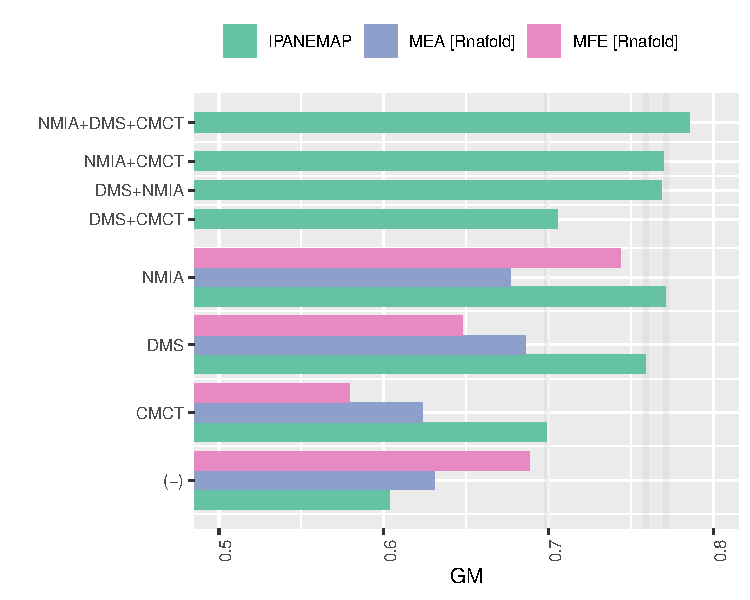
\includegraphics[trim=.5cm .3cm .2cm .2cm, clip, width=\linewidth]{graphs/cordero_mean}}\\}
	
	\caption{Averaged GM values for structures  predicted using \OurTool{} for subset combination of probing data. MFE and MEA structures, as computed by RNAfold, are included as controls in the absence of probing data, and for mono-probing.}
	\label{cordero1}
\end{figure}


Interestingly, in the absence of probing data, MFE predictions are generally dominant on this dataset, trailed by the MEA, and followed by \OurTool which, in this setting, devolves into the Ding-Lawrence algorithm~\citep{Ding2003}. However, whenever probing reactivities are available, the single centroid returned by \OurTool always achieves higher GM values (Avg: $70\%$) than both MEA (Avg: $62\%$) and MFE  (Avg: $58\%$), whose relative performances depend on the probing reagent.%la moyenne sur les 6 ARNS et sur les 3 reactifs
Interestingly, the quality of MFE and MEA predictions does not systematically benefit from additional probing data. Indeed, for half of the reagents and methods, the average GM obtained in the presence of a single reagent is lower than in the absence of probing data. Also, the impact of single probing data varies greatly across the three reagents, and the GE values of predictions respectively informed by CMCT, DMS and NMIA are ordered increasingly for all approaches, except for a minor reversal of DMS and NMIA in MEA mode.



The joint analysis of pairs of probing conditions seems to average the quality of predictions. Any combination of probing combinations yields a GM value that is always greater than the worst-performing condition in the pair, yet worse than the best-performing alone. Interestingly, the addition of the worst performing condition (CMCT), does not equally affect the performances of DMS ($76\% \to 70.5\%$) %DMS \to DMS+CMCT
and NMIA  ($77.1\% \to 76.9\%$), %NMIA \to NMIA+CMCT
despite the latter conditions inducing similar GM values when considered alone. Indeed, CMCT+DMS yields GM values that are only remotely better than the worst-performing CMCT alone  ($70\% \to 70.5\%$), while CMCT+NMIA greatly outperforms CMCT alone  ($70\% \to 76.9\%$), almost matching the performance of the NMIA alone ($77.1\%$). It is also worth mentioning that NMIA+CMCT, combining the best and worst conditions, achieves a better combined performance than DMS+NMIA, the two best mono-probing conditions. This hints towards some level of complementarity between probing conditions, as already suggested by recent analyses \citep{Yu2018} and supported by further analyses in this paper.

Remarkably, the combination of the three conditions leads to the best overall predictions, averaging $78.5\%$ GM.
This improves by $8.5\%$, $2.7\%$ and $1.4\%$ the average predictions achieved using CMCT, DMS and NMIA respectively.
%CMCT/DMS/NMIA :0.6988333333/0.7588333333/0.771
Table~\ref{fig:glycine_example} illustrates the incremental refinement of \OurTool predictions for a glycine riboswitch upon increasing the number of structures.
 




%\clearpage



\subsection{\OurTool typically outperforms state-of-the-art predictive methods on single probing data}
%Mono-probing Mathews (Hadjim)
%* On est meilleur sur la version courante de RSample
%* Multi conformation
We assess the predictive capacities of \OurTool in a classic setting where a single probing condition is available, and compare its performances against \Software{RSample} software recently introduced by~\cite{Mathews2017}, \Software{RSample} relies on a sampling/clustering method developed independently from the current work. It was shown to perform favorably against a comprehensive collection of state-of-the-art methods in probing-guided structure prediction, including \Software{RME}~\citep{Wu2015}, \Software{RNAprob}~\citep{Deng2016}, \Software{RNAprobing}~\citep{Washietl2012}, \Software{RNAsc}~\citep{Zarringhalam2012} and the \Software{fold} utility from the \Software{RNAstructure} suite~\citep{Reuter2010}.
We consider the dataset of hajdin~\emph{et al}, which consists of 24 RNAs of lengths ranging from 47 to 500 nucleotides, all believed to fold into a unique documented conformation. 

\begin{figure}
	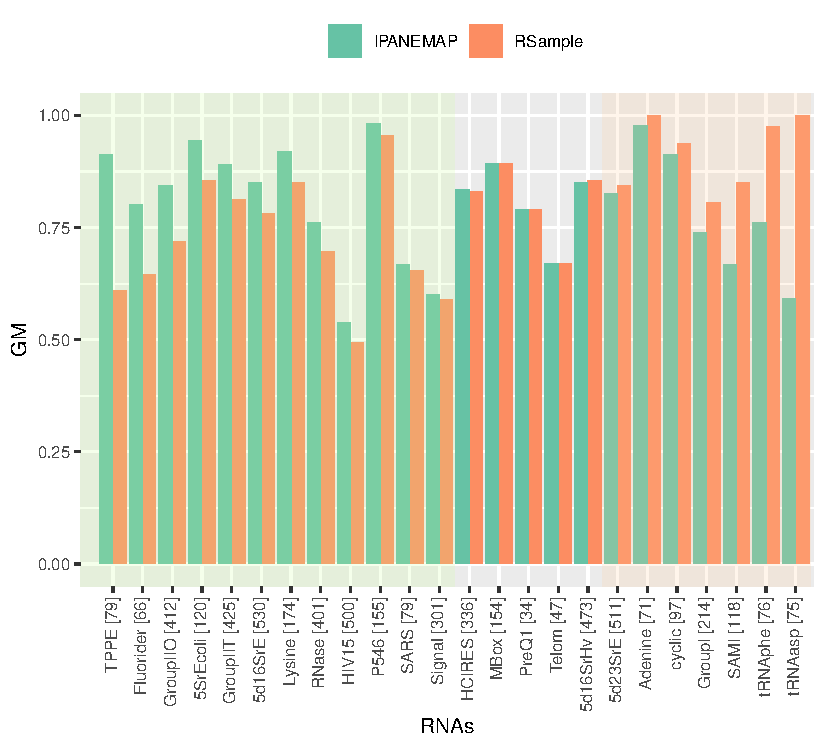
\includegraphics[width=\linewidth]{graphs/RsampleVsIPANEMAP/Accuracy}
	\caption{Geometric mean of positive predictive value and sensitivity achieved by the predictions of \OurTool{} and \Software{Rsample} over the Hadjin\etal\cite{Hajdin2013} data set, consisting of 24 RNAs (RNA length indicated within square brackets). \label{fig:Vsrsample}}
\end{figure}

We executed \OurTool with default parameters, producing 1~000 structures per sample for both software. The Pareto-optimality always implies a single returned cluster/structure in the case of a single probing condition. 
We also executed \Software{RSample} with default parameters, also returning a single structure for each sequence. 
We computed and report in Figure~\ref{fig:Vsrsample} the individual Geometric Means (GM) associated with predicted structures.


%\paragraph{Results description}
A first observation is that \OurTool generally outperforms \Software{Rsample}. It averages $80.1\%$ GM as opposed to $68\%$ for its competitor.  Out of the 24 considered RNAs, \OurTool outperforms its competitor for 16 out of the 24 RNAs, achieves similar performances for 2 of them, and is dominated for the remaining 6 cases. Whenever dominant, \OurTool achieves an average GM score of $82\%$, dominating by $32.8\%$ its competitor, while being dominated by $3.5\%$ over the remaining examples (including ties). 
%Difference<-c(IPANEMAP-Rsample)
%> sum(Difference[1:18])
%[1] 3.17
%> sum(Difference[19:24])
%[1] -0.382
Remarkably, \OurTool predicts secondary structures much more consistently than its competitor. 
It ensures GM that are greater than 50\% in all cases, and even exceeds 60\% over all except for the yeast tRNA, encoding the Aspartic acid and HIV1 5' pseudoknot domain. The standard deviation of GM for \OurTool is $12.5\%$, compared to the larger value of $21\%$ for \Software{Rsample} predictions.


%\paragraph{Discussion}



%Remarques These :
%\begin{itemize}
%  \item Fabrice : Y a t il une raison pour laquelle on est les meilleurs ?
%\end{itemize}
This observed discrepancy is somewhat surprising, given that \OurTool and \Software{Rsample} share the same sampling/clustering based modeling. However, the two methods differ substantially whenever a single conformation is detected, in which case \Software{Rsample} switches to a simple MEA prediction, whereas \OurTool{} always proceeds with an iterative clustering. This allows \OurTool{} to consider a larger number of clusters, which we believe helps eliminating structural outliers, leading to the election of a better final centroid structure. 


%\clearpage


\subsection{Comparing and exploiting multiple probing conditions: A case study on the Lariat capping ribozyme}

\newcommand{\Bull}[1]{{\sffamily #1}~\raisebox{1pt}{\tikzcircle[black, fill=cluster#1]{3pt}}}

\newcommand{\BullLab}[1]{Cluster \Bull{#1}}

\colorlet{clusterA}{SeaGreen}
\colorlet{clusterB}{Yellow}
\colorlet{clusterC}{gray}
\definecolor{clusterD}{HTML}{AFAFE9}
\colorlet{clusterE}{OliveGreen}
\colorlet{clusterF}{blue!90!black}
\colorlet{clusterG}{Orange}
\colorlet{clusterH}{SeaGreen!40}

\begin{figure*}
	{\centering {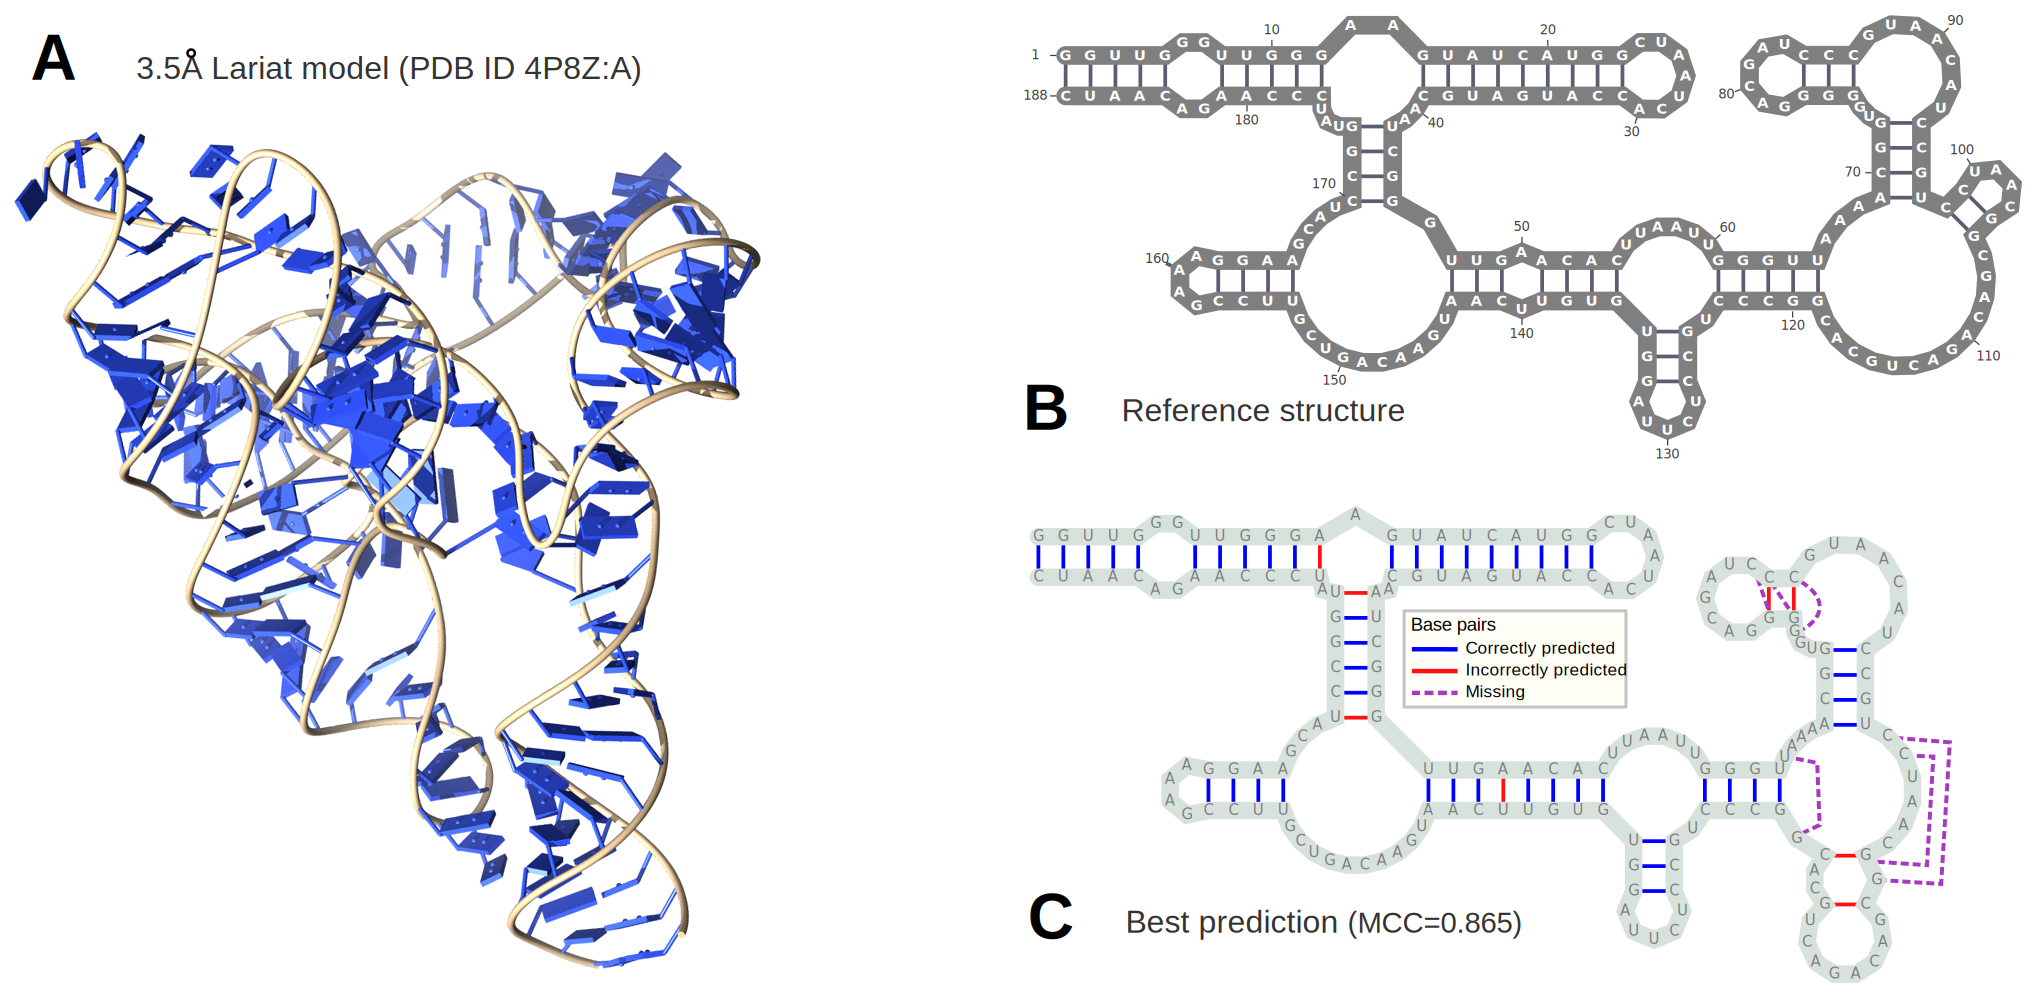
\includegraphics[width=.9\linewidth]{graphs/didy/didy}}\\}
	
	\caption{Model of the Lariat capping ribozyme in {\itshape Didymium iridis} (A -- Meyer\etal\cite{Meyer2014}), secondary structure as annotated by \Software{DSSR} (B -- pseudoknot ommitted) and \OurTool first-ranking prediction (C.) from 8 maximally-diverging probing conditions (NMIAMg, 1M7ILU3Mg, NAIMg, 1M7, CMCTMg,1M7ILU3,1M7Mg). }
\end{figure*}



\paragraph{Comparison and clustering of conditions.}
Faced with diverse probing conditions, we first assess the compatibility of the conclusions drawn from different probing data, including the probing-free run of \OurTool as a control. We use the methodology described in subsection~\ref{sec:dotplots} and, for each condition, compute the base pair probability distribution (aka dot-plot) in the  pseudo-Boltzmann ensemble, induced by the reactivity profile. We then computed the ensemble distance, the squared Euclidian distance between dot plots, for each pair of conditions. Figure~\ref{fig:PCA} summarizes the pairwise distance, projected onto a 2D surface by a principal component analysis.


\begin{figure}
	{\centering 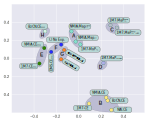
\includegraphics[width=\linewidth]{graphs/didy/PCA}\\}%, trim= 3.5cm .5cm 1cm 0,clip]
	
	\caption{2D spatial representation of conditions, computed by Principal Component Analysis (PCA) to optimally reflect pairwise ensemble distances between conditions. Colors and grayed areas indicate clusters of conditions.}\label{fig:PCA}
\end{figure}

A visual inspection of Figure~\ref{fig:PCA} suggests the presence of 8 clusters. In order to objectively build groups of compatible conditions, we performed a k-mean clustering using \Software{scikit-learn}, setting k to 8, and obtained the clusters highlighted in Figures~\ref{fig:biclustering} and \ref{fig:PCA}.  We obtain the following clusters:
\begin{itemize}\setlength{\itemsep}{0pt}\setlength{\parskip}{.1em}	
\item \BullLab{A}: 1M7ILU, NMIA, and NMIAMg;
\item \BullLab{B}: 1M7CE, NMIACE, BzCN, and NAI;
\item \BullLab{C}: 1M7ILU3Mg and 1M7ILUMg;
\item \BullLab{D}: 1M7ILU3;
\item \BullLab{E}: NMIAMgCE and 1M7MgCE;
\item \BullLab{F}: DMSMg and probing-free;
\item \BullLab{G}: CMCTMg and NAIMg;
\item \BullLab{H}: BzCNMg.
\end{itemize}
The predicted clusters are generally consistent with the ordering resulting from a spectral biclustering, implemented in \Software{scikit-learn} and executed with default parameters, as illustrated by Figure~\ref{fig:glycine_example}. 

The average ensemble distance and PCA visualization support a status of outliers for conditions in the cluster \Bull{B} (1M7CE, NMIACE, BzCN and NAI).  We hypothesize that such conditions may be either representative of alternative conformations, or be altogether erroneous. Consequently, we will single out these two clusters within our detailed analysis of the multi-probing performances.








\begin{figure}
	{\centering 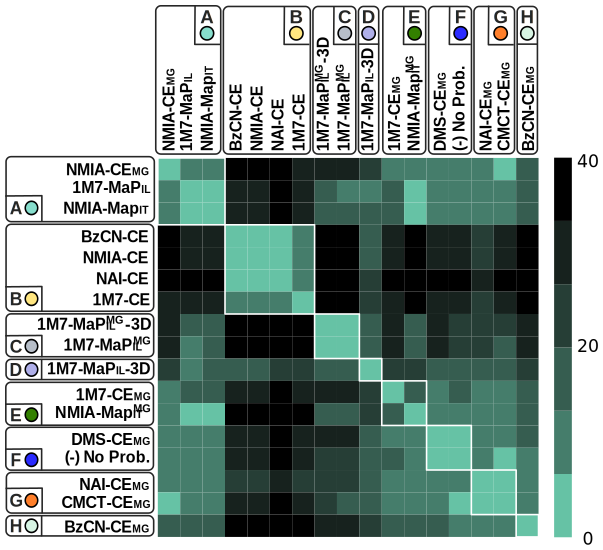
\includegraphics[width=\linewidth]{graphs/didy/bi_clustering}\\}%, trim= 3.5cm .5cm 1cm 0,clip]
	
	\caption{Discretized ensemble distance induced by conditions. Conditions ordered by spectral biclustering. Conditions regrouped within clusters by k-mean clustering appear as blocks on the x and y axis.}\label{fig:biclustering}
\end{figure}






%\clearpage

\paragraph{Assessment of predictions informed by individual probing conditions (mono).}
%First, we assess the individual performance of each probing condition considered as the sole source of structural constraints.  Then, analyze outperforming experimental conditions that ensure more accurate predictions, and spot \Def{outlier} conditions which, on the contrary, seem to increase the noise level, consequently leading to lower prediction performances for \OurTool{}. 



For each probing condition, we run \OurTool{} on a single source of probing data, using a sample size of $1~000$ structures. For the sake of reproducibility, we executed \OurTool{} $10$ times for each condition. We report in Table~\ref{tab:thermo-ipan} the MCC values achieved by our prediction, averaged over the $10$ runs, along with the MCCs obtained by running \Software{RNAfold} with default parameters in energy minimization (MFE) and Maximum Expected Accuracy (MEA) modes.


The predictive performances of \OurTool averages a 70.5\% MCC, compared to 68.5\% and 68\% average MCC for MEA and MFE predictions respectively. The stability of predictions across conditions are comparable for all \OurTool, MEA and MFE-driven predictions (std dev. of 8\%). Excluding the outliers of cluster \Bull{B} improves the average MCC to 74\%.

Over the fourteen conditions, we observe a large discrepancy in the capacity of the experimental setup to inform predictions, with MCCs ranging from above 80\% (NMIA, NMIAMg, 1M7ILU and 1M7ILUMg) to around 60\% (NAI, BzCN, 1M7CE and NMIACE). These values are much better than those achieved in the absence of probing data (51\% MCC). Such values can be interpreted as indicate of good quality predictions. Indeed, it should be reminded that the MCC is a stringent metrics, taking values between -100\% and 100\%, 0\% being the expected MCC of a "coin tossing" random predictor. The lowest MCC value of 60\% is, in particular, equally consistent with Sensitivity/PPV values of 60\%/60\%, 80\%/46\% or 45\%/82\%.

Unsurprisingly, the presence/absence of Magnesium during the probing impacts the predictions, with an observed drop from an average 73\% MCC in the presence of Mg$^\text{2+}$ to 67\% MCC in the absence of Mg$^\text{2+}$. However, while the poorly performing conditions of cluster \Bull{B} are Mg$^\text{2+}$ free, some of the most informative profiles (1M7ILU and NMIA) were obtained in absence of Mg$^\text{2+}$.
An even more drastic change of performances can be observed in the comparison of the average MCC of mutation-inducing reagents (78\%) with stop-inducing ones (66\%). 

\begin{table}
	\Heatset{min=60,   
		max=83,   
		max colour=Aquamarine3, % colour at maximum
		min colour=BadCol,      % colour at minimum
		Min colour=BadCol, % colour for values below min
		Max colour=Aquamarine3   % colour for values above max
	}
	\newcommand{\Mut}{Mut}
	\newcommand{\Stop}{Stop}
	\newcommand{\Mg}{$\bullet$}
	\newcommand{\NoMg}{$\circ$}
	
	{\centering
			\begin{adjustbox}{max width=\linewidth}
		\begin{tabular}{@{}lcccHHH}
			\toprule
			                            &          &         &           & \multicolumn{3}{@{}c@{}}{MCC\%}                                                  \\
			Condition                   &  Clust.  &  Tech.  & Mg$^{2+}$ & \multicolumn1l{\relsize{-1}\OurTool} & \multicolumn1l{MFE} & \multicolumn1l{MEA} \\ \midrule
			1M7ILUMg                    & \Bull{C} &  \Mut   &    \Mg    & 85                                   & 82                  & 82                \\
			1M7ILU                      & \Bull{A} &  \Mut   &   \NoMg   & 84                                   & 82                  & 84                \\
			NMIAMg                      & \Bull{A} &  \Mut   &    \Mg    & 81                                   & 80                  & 80                \\
			NMIA                        & \Bull{A} &  \Mut   &   \NoMg   & 80                                   & 69                  & 69                \\
			1M7ILU3Mg                   & \Bull{C} &  \Mut   &    \Mg    & 74                                   & 75                  & 75                \\
			NMIAMgCE                    & \Bull{E} &  \Stop  &    \Mg    & 73                                   & 72                  & 73                \\
			NAIMg                       & \Bull{G} &  \Stop  &    \Mg    & 73                                   & 68                  & 70                \\
			BzCNMg                      & \Bull{H} &  \Stop  &    \Mg    & 71                                   & 68                  & 54                \\
			1M7MgCE                     & \Bull{E} &  \Stop  &    \Mg    & 70                                   & 69                  & 70                \\
			CMCTMg                      & \Bull{G} &  \Stop  &    \Mg    & 70                                   & 68                  & 73                \\
			1M7ILU3                     & \Bull{D} &  \Mut   &   \NoMg   & 64                                   & 56                  & 61                \\
			DMSMg                       & \Bull{F} &  \Stop  &    \Mg    & 63                                   & 66                  & 67                \\
			NMIACE                      & \Bull{B} &  \Stop  &   \NoMg   & 61                                   & 60                  & 60                \\
			1M7CE                       & \Bull{B} &  \Stop  &   \NoMg   & 60                                   & 61                  & 61                \\
			BzCN                        & \Bull{B} &  \Stop  &   \NoMg   & 60                                   & 59                  & 59                \\
			NAI                         & \Bull{B} &  \Stop  &   \NoMg   & 60                                   & 59                  & 59                \\ \midrule
			Avg Technology              &          &  \Mut   &  $\star$  & 78                                   & 74                  & 75                \\
			                            &          &  \Stop  &  $\star$  & 66                                   & 65                  & 65                \\
			Avg -/+ Mg$^{2+}$           &          & $\star$ &   \NoMg   & 67                                   & 64                  & 65                \\
			                            &          & $\star$ &    \Mg    & 73                                   & 72                  & 71.5               \\ \midrule
			{\bfseries Average overall} &          & $\star$ &  $\star$  & 70.5                                 & 68                  & 68.5               \\ \bottomrule
			                            &          &         &           &
		\end{tabular}
		\end{adjustbox}\\[1em]}
	
	%data are from multiprobing7 
	\caption{Comparison of predicted secondary structures for the \didy{} obtained with \OurTool{} and computational methods from a mono-probing experiment. Averaged MCC of structures predicted with \OurTool{} and with classic deterministic alternatives. The structure was probed in presence (\Mg) or absence (\NoMg) of Magnesium, using either stops (\Stop) or mutations (\Mut) inducing technologies.
	}
	\label{tab:thermo-ipan}
\end{table}




\begin{figure}
	\newcommand{\W}{.73}
	{\centering\begin{tabular}{@{}c@{}c@{}c@{}}
			{\sf {\bfseries A} -- \relsize{-1}Bi-probing MCC \emph{vs} Min MCC of mono-probing}\\
			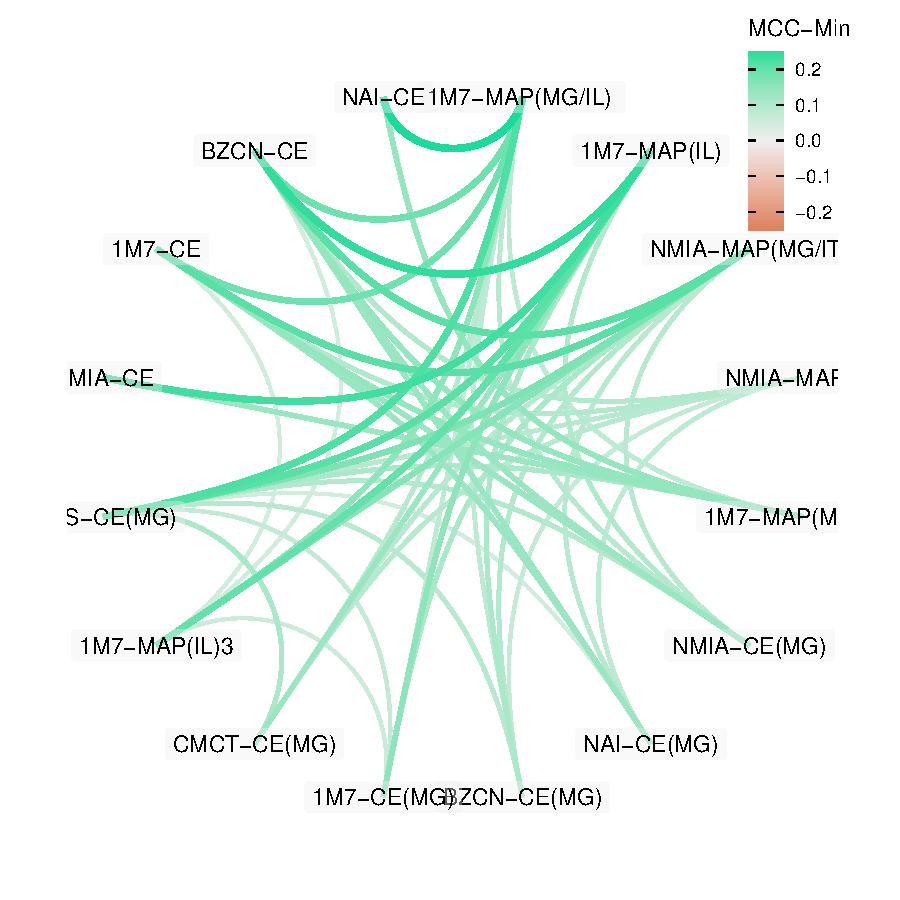
\includegraphics[width=\W\linewidth,trim=1cm 1cm .8cm .3cm,clip]{graphs/didy/MCC-vs-Min}\\[.5em]
			{\sf {\bfseries B} -- \relsize{-1}Bi-probing MCC \emph{vs} Average MCC of mono-probing}\\
			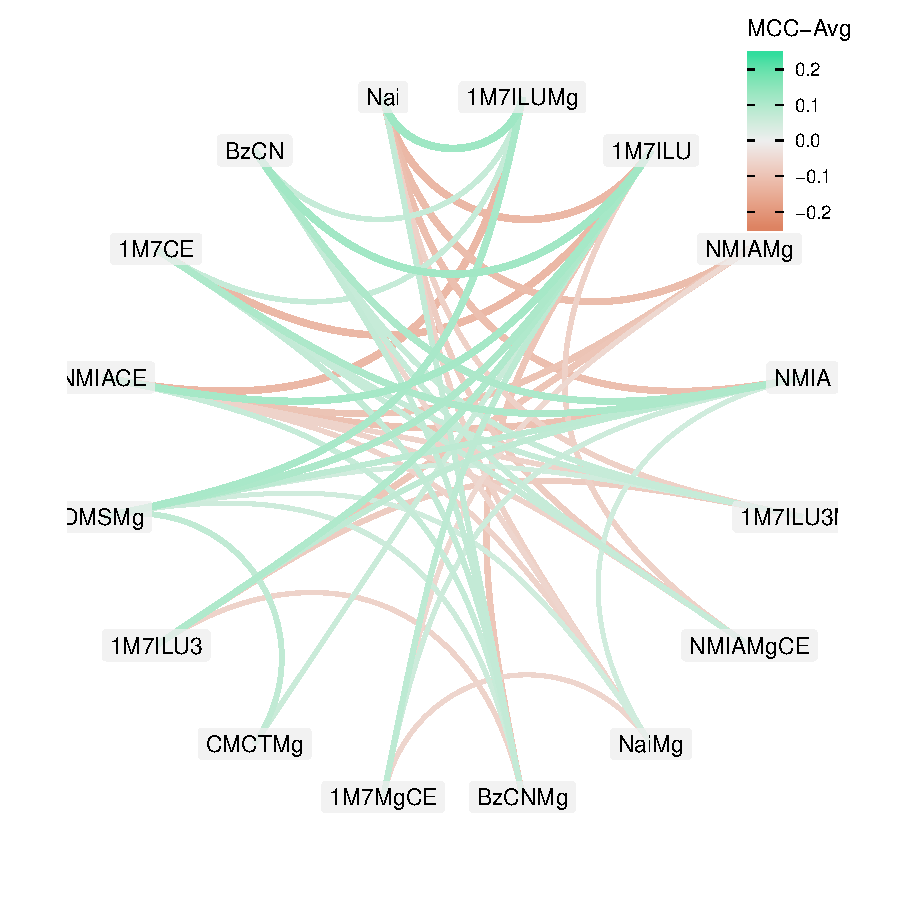
\includegraphics[width=\W\linewidth,trim=1cm 1cm .8cm .3cm,clip]{graphs/didy/MCC-vs-Avg}\\[.5em]
			{\sf {\bfseries C} -- \relsize{-1}Bi-probing MCC \emph{vs} Max MCC of mono-probing}\\
			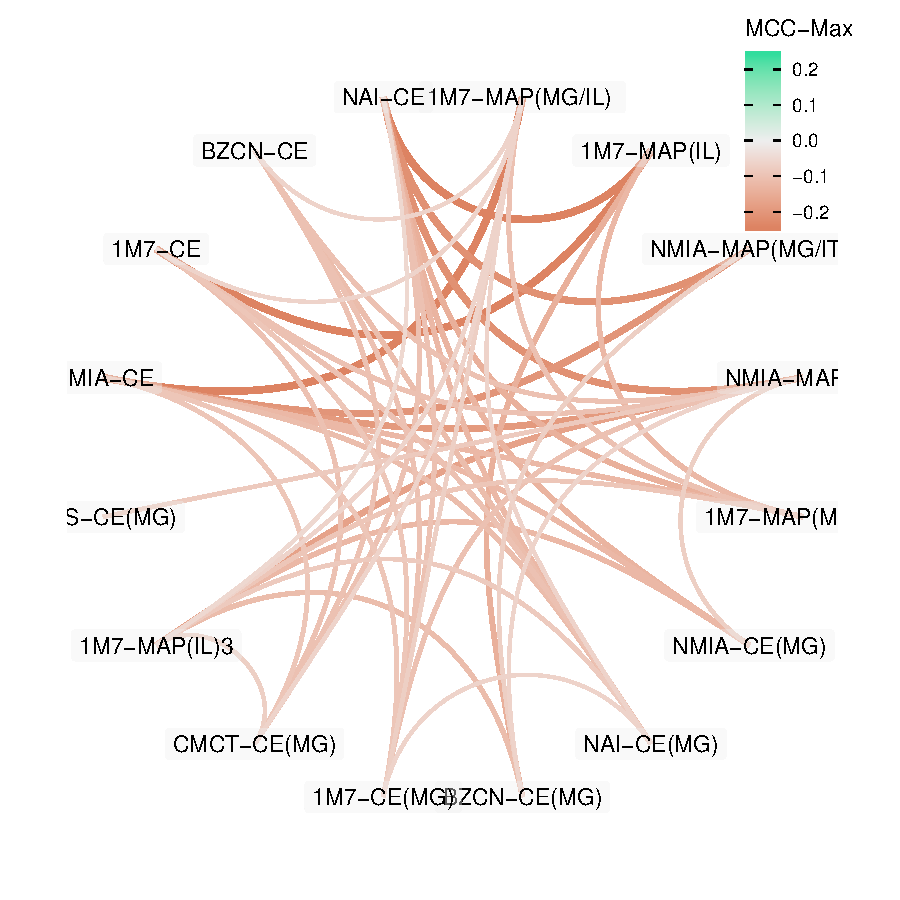
\includegraphics[width=\W\linewidth,trim=1cm 1cm .8cm .3cm,clip]{graphs/didy/MCC-vs-Max}\\
		\end{tabular}\\}
	\caption{Shift in \OurTool{} predictive capacity (MCC) observed upon considering two conditions, compared to the worst ({\sf\bfseries A}),  average ({\sf\bfseries B}) 
		and best ({\sf\bfseries C}) 
		predictions achieved for mono-probing conditions. Green and red edges indicate enhanced and degraded predictions respectively compared to the reference (Min% 
		, Max 
		or Average of conditions). Thickness indicates absolute shift value (only values above 5\% reported for readability).\label{fig:pairwise}}
\end{figure}

\paragraph{Bi-probing mitigates the influence of outliers, but generally fails to improve predictions quality.}
We turn to a systematic exploration of the predictive capacities of bi-probing analyses, based on pairs of probing profiles, and attempt to quantify their impact on \OurTool predictions. For each pair and triplets of conditions, we executed \OurTool using 1~000 samples per condition, and considered the first returned structure. We then computed the associated MCC, and compare it with the MCC of the worst performing condition (Min), best performing condition (Max) and average MCC over the single conditions experiments. A summary of the results over pairs is shown in Figure~\ref{fig:pairwise}. 

A superficial inspection of the resulting MCCs appears to confirm the conclusions of Section~\ref{sec:cordero}. Indeed, considering two conditions leads to predictions whose quality fall between the worst and the best one, while being generally close to the average. More precisely, the average MCC value of pair-informed predictions remains at 70.7\%, improving only by 0.2\% over the average MCC of mono-probing predictions. Pair-informed predictions are marginally more reliable, with the median MCC increases to 72.5\% MCC from 70.5\% for mono-probing predictions. However, outliers strongly impact this picture, and ignoring the conditions in cluster \Bull{B} increases the average MCC to 75.1\%, while unsurprisingly decreasing the standard deviation (8.6\% $\to$ 6.5\%).

Compared to the minimum MCC of the pair, the MCC of bi-probing predictions is improved by 5.3\% on average over the MCC of the worst-performing conditions. Pair MCCs exceed their associated min. MCC by at least 5\% in 47 pairs out of the 120 possible pairs, while never being dominated by 5\%. 

Bi-probing tends to perform similarly as the average of the two mono-probing conditions, with an average MCC improvement of 0.2\%. However, for 56 out of the 120 possible pairs, the bi-probing conditions exhibits an improvement of at least 1\% over the average, while a decay of at least 1\% is observed for 46 out of the remaining 64 pairs. Such a decay can partly be attributed to the disruptive effect of the outliers from cluster \Bull{B}, involved in 35 of the 46 observed loss of predictive performance. Moreover, removing this cluster induces an average MCC improvement of 1.1\%.

Predictions informed by two conditions remain, however, generally dominated by the best performing condition of the pair. On average, the MCC of the best condition is 4.9\% higher than the one achieved by bi-probing analysis. 
Outliers in cluster \Bull{B} are partly responsible for this situation, and their removal reduces the average MCC decay to 3.3\%. Moreover, for 9 pairs of conditions, the bi-probing analysis produces MCC that are at least 1\% better than the best of its two conditions, but these encouraging examples are generally dominated by 66 examples where the pair performs more than 1\% worse than the best mono-probing condition.

\paragraph{Considering three conditions yields improvement over the average performance of the triplet.}
Increasing the number of conditions to three boosts the average MCC to 72.3\% and even reaches 76.5\% over triplets that do not contain conditions from cluster \Bull{B}. The MCC gain over the worst condition in the triplet reaches 9.1\% on average.  Predictions are also more consistently good, with a median MCC of \%73.4. Disregarding conditions in cluster \Bull{B} does stabilizes the quality of prediction (stdev 8.4\% $\to$ 5.5\%), while increasing the average MCC to 77.4\%.

Compared to bi-probing, MCC values achieved by integrating triplets of conditions now indicate a clear gain over the average performances of individual conditions, supporting a notion of complementarity between experiments. Indeed tri-probing experiments lead to an average +1.7\% MCC improvement (median +2.6) over the average of mono-probing prediction in the triplet. The gain of quality is widespread, and observed for 65\% of the triplets. Finally, 39 triplets were found to induce MCC values greater than 83\%.

The enhanced performances of tri-probing over bi-probing are consistent with the \emph{voting} principle underlying the clustering used in \OurTool. Indeed, in a bi-probing setting, a single outlier condition, such as NAI, may entirely determine the final structure, due to its predictions being very tightly concentrated around a, presumably erroneous, structure. In the presence of three or more conditions, however, clusters resulting from an outlier condition typically end up being dominated, in the Pareto front, by compatible sets of structures originating from the pseudo-Boltzmann ensembles of alternative conditions. It follows that the influence of outliers over the final prediction remains limited.

%\clearpage


\begin{table}[h]
	\Heatset{min=60,   
		max=83,   
		max colour=Aquamarine3, % colour at maximum
		min colour=BadCol,      % colour at minimum
		Min colour=BadCol, % colour for values below min
		Max colour=Aquamarine3   % colour for values above max
	}
    \newcommand{\Q}{\relsize{-1}}

	{\centering
		\begin{adjustbox}{max width=\linewidth}
			\begin{tabular}{@{}llHH@{}}
				\toprule
				&                                           & \multicolumn{2}{@{}c@{}}{MCC\%}                     \\
				& Conditions                                & \multicolumn{1}{@{}c@{}}{\Q{}Joint} &  \multicolumn{1}{@{}c@{}}{\Q{}Mono} \\ \midrule
				{Cluster \Bull{A}} & NMIAMg, 1M7ILU, NMIA                       & 80                  & 82                      \\
				& NMIAMg, 1M7ILU                             & 82                  & 82                      \\
				& 1M7ILU, NMIA                               & 82                  & 82                      \\
				& NMIAMg,  NMIA                              & 80                  & 80                      \\ \midrule
				{Cluster \Bull{B}}                         & Nai, BzCN, 1M7CE, NMIACE                   & 60                  & 60                      \\
				& Nai, BzCN, 1M7CE                           & 60                  & 60                      \\
				& Nai, BzCN, NMIACE                          & 61                  & 60                      \\
				& Nai, 1M7CE, NMIACE                         & 61                  & 60                      \\
				& BzCN, 1M7CE, NMIACE                        & 61                  & 60                      \\
				& Nai, BzCN                                  & 60                  & 60                      \\
				& Nai, 1M7CE                                 & 59                  & 60                      \\
				& Nai, NMIACE                                & 60                  & 60                      \\
				& BzCN, 1M7CE                                & 61                  & 60                      \\
				& BzCN,NMIACE                                & 60                  & 60                      \\
				& 1M7CE, NMIACE                              & 62                  & 61                      \\ \midrule
				{Cluster \Bull{C}}                         & 1M7ILUMg, 1M7ILU3Mg                        & 82                  & 80                      \\ \midrule
				{Cluster \Bull{E}} & 1M7MgCE, NMIAMgCE                          & 73                  & 72                      \\ \midrule
				{Cluster \Bull{G}}                         & NaiMg, CMCTMg                              & 73                  & 72                      \\ \bottomrule
				%				\midrule
				%				{All 16 conditions} & .80                   & .70                       \\ \bottomrule
			\end{tabular}
		\end{adjustbox}
		\\}
	\caption{Predictions do not benefits from the joint consideration of similar conditions. For each cluster, all subsets of conditions in the cluster are considered, and the MCC of the resulting prediction ('Joint') is compared to the average MCC of predictions performed with individual conditions independently ('Mono'), revealing little improvement.}\label{fig:similarconds}
\end{table}

\paragraph{Similar conditions do not contribute to the quality of predictions.} 
Our distance assessment and clustering on conditions reveals groups of conditions that are highly compatible in their conclusions, while others seem to include highly diverging structural information. While some outlier conditions, such as those of cluster \Bull{B}, easily stand out as erroneous, the results of our systematic analysis of pairs and triplets supports a notion of \Def{complementarity between conditions}. Under this assumption, downstream analyses are more likely to benefit from the presence of highly diverging probing experiments, than the accumulation of similar, arguably redundant, profiles. 

A first test of this hypothesis consists in executing \OurTool{} on every subset of conditions within clusters, and consider the quality of predictions (MCC). 
Note that our similarity notion and clustering of conditions is purely based on the ensemble features, and does not explicitly consider the MCC of individual conditions. 
As expected, compared to the average MCC over associated mono-probing analyses, a joint consideration of similar conditions only induces limited progress over single probing analyses (between -1\% and +1\%), leading to an modest average improvement (+0.2\% average MCC). This is consistent with the notion that supplementing a probing-based modeling with compatible conditions provides very little additional information, leading to a limited contribution of similar conditions. 



\paragraph{Considering diverse conditions improves and stabilizes the quality of predictions.} 
Having established the redundant nature of similar conditions, and their limited contribution to downstream modeling, we turn to an analysis of conditions across clusters.  We run \OurTool{} the quality of predictions obtained by choosing a single condition in each of the 8 clusters. We consider any possible combination, except for the outlier cluster~\Bull{B}. Instead, we only consider the impact of including NAI to each combination.

The results, summarized in Table~\ref{fig:differentconds}, demonstrate a clear advantage of including diverse conditions, leading to an average MCC value of 77\% in the absence of condition from cluster \Bull{B}. Those performances compare favorably against the 72\% MCC achieved on average by individual conditions, and reveal a remarkable stability, including a 5\% standard deviation, and a degradation in only two out the 24 tested cases ($\sim$1\% decay in both cases).  A similar trend can be observed in the, arguably disruptive presence of NAI, inducing an 72\% average MCC, albeit with an increased standard deviation of 9\%.

Finally, the consideration of four triplets of diverse conditions allow us to reach our best prediction, achieving 85.3\% MCC. Meanwhile, considering the 16 conditions together yields a 80\% MCC value, increasing to 83\% in the absence of the four outlier conditions of cluster \Bull{B}. These results confirm that the strategy used by \OurTool{} is able to exploit the complementary information provided by multiple conditions, contributing to better predictions.

	\begin{table}[h]
	\Heatset{min=60,   
		max=83,   
		max colour=Aquamarine3, % colour at maximum
		min colour=BadCol,      % colour at minimum
		Min colour=BadCol, % colour for values below min
		Max colour=Aquamarine3   % colour for values above max
	}
    \newcommand{\MC}[1]{\multicolumn{1}{@{}c@{}}{#1}}
    \newcommand{\MCB}[1]{\multicolumn{2}{@{}c@{}}{#1}}
    \newcommand{\Q}{\relsize{-1}}

	\begin{adjustbox}{max width=\linewidth}
		\begin{tabular}{@{}llllHHHH@{}}
			\toprule
			\multicolumn{4}{@{}l@{}}{}                                    & \multicolumn{4}{@{}c@{}}{MCC\%}\\
			\multicolumn{4}{@{}l@{}}{Conditions in individual clusters}                                    & \MCB{-NAI} & \MCB{+NAI} \\
			\Bull{A} & \Bull{C} & \Bull{E} & \Bull{G}   & \MC{\Q Joint} & \MC{\Q Mono}  & \MC{\Q Joint}       & \MC{\Q Mono}      \\ \midrule
			\Q NMIAMg          & \Q 1M7ILUMg        & \Q 1M7MgCE          & \Q NaiMg             & 84       & 72       & 83             & 71           \\
			\Q NMIAMg          & \Q 1M7ILUMg        & \Q 1M7MgCE          & \Q CMCTMg            & 75       & 72       & 82             & 71           \\
			\Q NMIAMg          & \Q 1M7ILUMg        & \Q NMIAMgCE         & \Q NaiMg             & 79       & 73       & 82             & 71           \\
			\Q NMIAMg          & \Q 1M7ILUMg        & \Q NMIAMgCE         & \Q CMCTMg            & 82       & 72       & 60             & 71           \\
			\Q NMIAMg          & \Q 1M7ILU3Mg       & \Q 1M7MgCE          & \Q NaiMg             & 70       & 71       & 60             & 70           \\
			\Q NMIAMg          & \Q 1M7ILU3Mg       & \Q 1M7MgCE          & \Q CMCTMg            & 70       & 70       & 72             & 69           \\
			\Q NMIAMg          & \Q 1M7ILU3Mg       & \Q NMIAMgCE         & \Q NaiMg             & 72       & 71       & 74             & 70           \\
			\Q NMIAMg          & \Q 1M7ILU3Mg       & \Q NMIAMgCE         & \Q CMCTMg            & 75       & 71       & 60             & 70           \\
			\Q 1M7ILU          & \Q 1M7ILUMg        & \Q 1M7MgCE          & \Q NaiMg             & 82       & 73       & 75             & 71           \\
			\Q 1M7ILU          & \Q 1M7ILUMg        & \Q 1M7MgCE          & \Q CMCTMg            & 84       & 72       & 60             & 71           \\
			\Q 1M7ILU          & \Q 1M7ILUMg        & \Q NMIAMgCE         & \Q NaiMg             & 73       & 73       & 60             & 72           \\
			\Q 1M7ILU          & \Q 1M7ILUMg        & \Q NMIAMgCE         & \Q CMCTMg            & 82       & 73       & 82             & 71           \\
			\Q 1M7ILU          & \Q 1M7ILU3Mg       & \Q 1M7MgCE          & \Q NaiMg             & 84       & 71       & 60             & 70           \\
			\Q 1M7ILU          & \Q 1M7ILU3Mg       & \Q 1M7MgCE          & \Q CMCTMg            & 70       & 71       & 84             & 70           \\
			\Q 1M7ILU          & \Q 1M7ILU3Mg       & \Q NMIAMgCE         & \Q NaiMg             & 74       & 72       & 60             & 70           \\
			\Q 1M7ILU          & \Q 1M7ILU3Mg       & \Q NMIAMgCE         & \Q CMCTMg            & 74       & 71       & 75             & 70           \\
			\Q NMIA            & \Q 1M7ILUMg        & \Q 1M7MgCE          & \Q NaiMg             & 82       & 72       & 75             & 71           \\
			\Q NMIA            & \Q 1M7ILUMg        & \Q 1M7MgCE          & \Q CMCTMg            & 83       & 72       & 82             & 70           \\
			\Q NMIA            & \Q 1M7ILUMg        & \Q NMIAMgCE         & \Q NaiMg             & 73       & 73       & 59             & 71           \\
			\Q NMIA            & \Q 1M7ILUMg        & \Q NMIAMgCE         & \Q CMCTMg            & 82       & 72       & 82             & 71           \\
			\Q NMIA            & \Q 1M7ILU3Mg       & \Q 1M7MgCE          & \Q NaiMg             & 73       & 71       & 82             & 69           \\
			\Q NMIA            & \Q 1M7ILU3Mg       & \Q 1M7MgCE          & \Q CMCTMg            & 70       & 70       & 73             & 69           \\
			\Q NMIA            & \Q 1M7ILU3Mg       & \Q NMIAMgCE         & \Q NaiMg             & 74       & 71       & 68             & 70           \\
			\Q NMIA            & \Q 1M7ILU3Mg       & \Q NMIAMgCE         & \Q CMCTMg            & 74       & 71       & 73             & 69           \\ \midrule
			                &                 &                  & Average           & 77       & 72       & 72             & 70           \\ \bottomrule
		\end{tabular}
	\end{adjustbox}\\
	\caption{Predictive performances of conditions across clusters, coupled with impact assessment of NAI.  For each experiment, a single condition is chosen from each cluster except for cluster \Bull{B}. Clusters \Bull{D}, \Bull{F} and \Bull{H}, each consisting of a single condition, contribute their sole condition, leading to the list of conditions  $\mathcal{M}$:=\{1M7ILU3, BzCNMg and DMSMg\}. 
		For each combination, the MCC of the predicted structural model is reported, as predicted from the conditions in the presence/absence of NAI ('Joint' columns). For each prediction, the average MCC value of mono conditions is reported as a baseline ('Mono' columns).
	}\label{fig:differentconds}
\end{table}

%
%	\begin{table}
%	\newcommand{\A}{90}
%	
%	\centering
%	\begin{adjustbox}{max width=\linewidth}
%		\begin{tabular}{@{}ccccccccc@{}}
%			\toprule
%			\rotatebox{\A}{\Bull{C} 1M7ILUMg} & \rotatebox{\A}{\Bull{D} 1M7ILU3} & \rotatebox{\A}{\Bull{A} 1M7ILU} & \rotatebox{\A}{\Bull{F} DMSMg} & \rotatebox{\A}{\Bull{E} NMIAMgCE} & \rotatebox{\A}{\Bull{G} CMCTMg} & \rotatebox{\A}{\Bull{H} BzCNMg} &      MCC      & Mono-Avg \\ \midrule
%			$\bullet$             &                                  &            $\bullet$            &           $\bullet$            &                                   &                                 &                                 & \textbf{.853} &   .77    \\
%			$\bullet$             &                                  &            $\bullet$            &                                &             $\bullet$             &                                 &                                 & \textbf{.853} &   .81    \\
%			$\bullet$             &                                  &                                 &           $\bullet$            &                                   &            $\bullet$            &                                 & \textbf{.853} &   .73    \\
%			$\bullet$             &            $\bullet$             &                                 &                                &                                   &                                 &            $\bullet$            & \textbf{.853} &   .73    \\ \midrule
%			$\bullet$             &            $\bullet$             &            $\bullet$            &           $\bullet$            &             $\bullet$             &            $\bullet$            &            $\bullet$            &      .83      &   .73    \\ \bottomrule
%		\end{tabular}
%	\end{adjustbox}\\
%
%	\caption{Yann would you please modify the structure in Figure 4 according to the new structure?}
%\end{table}
%\begin{table}
%	\centering
%	\begin{adjustbox}{max width=.5\textwidth}
%		\begin{tabular}{@{}llllll@{}}
%			\toprule
%			Description & MCC & Mono-Avg\\
%			\midrule
%			12 conditions& {\bfseries.83}&.74 \\
%			{\em All 16 conditions} &	\textbf{.8}& .705\\
%			&	\textbf{.6}& \\
%			\bottomrule
%		\end{tabular}
%	\end{adjustbox}\\
%
%	\caption{Report the best possible score; + all conditions}
%\end{table}
%%

%\begin{figure*}
%\begin{adjustbox}{max width=\linewidth}
%  \begin{tabular}{ll}
% Seq & \tt {GGUUGGGUUGGGAAGUAUCAUGGCUAAUCACCAUGAUGCAAUCGGGUUGAACACUUAAUUGGGUUAAAACGGUGGGGGACGAUCCCGUAACAUCCGUCCUAACGGCGACAGACUGCACGGCCCUGCCUCUUAGGUGUGUUCAAUGAACAGUCGUUCCGAAAGGAAGCAUCCGGUAUCCCAAGACAAUC
%} \\
% 
% NATIVE &  \tt {(((((..(((((..(((((((((.......)))))))))..((((.(((.((((......(((((...((((..(((......))).......))))((....)).............))))).(((.....))))))).)))..........((((....))))....))))...)))))..)))))} \\
%
%.865 &\tt{(((((..((((((.(((((((((.......))))))))).((((((((((((((......((((....((((...((.......)).......))))......(.(........)..).)))).(((.....)))))))))))..........((((....))))...)))))).))))))..)))))}\\
% \\
%\end{tabular}
%\end{adjustbox}
%\caption{Content: 3D didymium + native structure + predicted base pairs}
%\end{figure*}
%\begin{figure}
%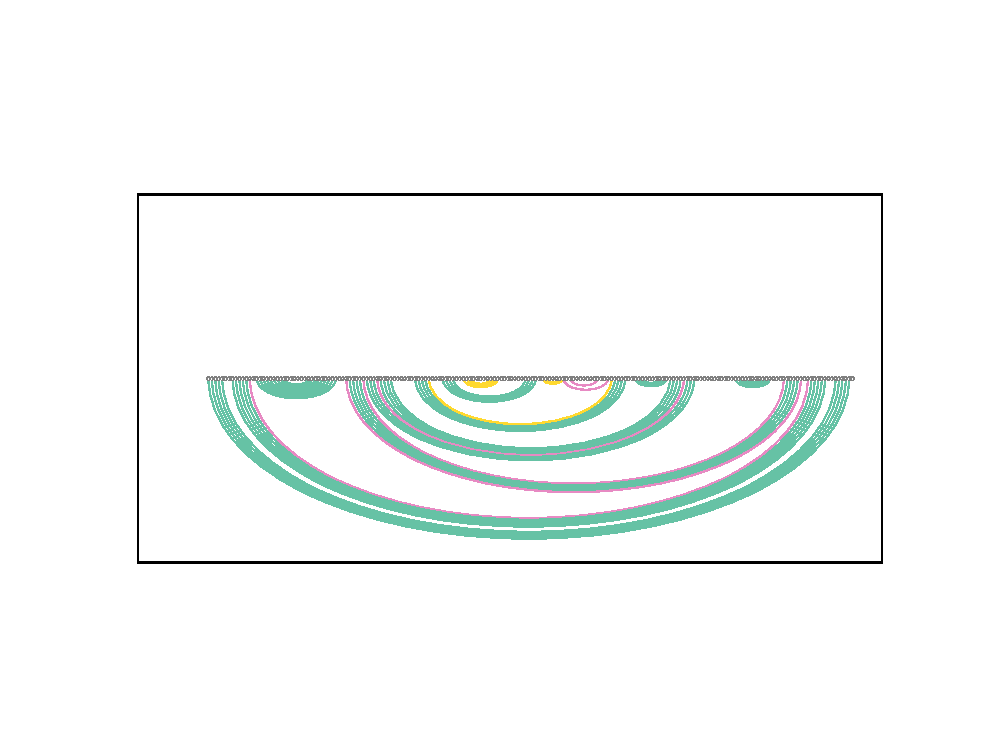
\includegraphics[width=\linewidth]{graphs/Arcs}
%\end{figure}
%\subsection{\OurTool{} yields reproducible predictions}
%\as{Which structure?}



\subsection{Supplementing wild-type profiles with random single mutants increases prediction quality}
In this final analysis, we decided to test the capacity of \OurTool to extract and exploit complementary information produced by the systematic probing of single-point mutants.
This approach may appear misguided, since single point mutants are expected to adopt different structures than the wild-type sequence. In fact, the conformational changes induced by mutations precisely constitute the signal that is exploited by downstream modeling pipelines~\cite{Cordero2015}. However, those changes are typically local, and the limited influence of outliers on \OurTool{} raises a hope that the benefit of including independently-produced conditions will outweigh the impact of noise introduced by local changes.

We generated 100 uniformly-distributed subsets consisting of 1, 2, 3 and 10 mutants extracted from the Cheng dataset~\cite{Cheng2017}, which we supplemented with the original wild-type sequence (WT).
For each set of probing profiles, we executed \OurTool{} with default parameters, using a sample size of 1~000 structures. 
We also analyzed the WT sequence alone, reproducing the analysis 100 times to compare the variability across sets of mutants to the one induced by stochastic aspects of our method. 
Finally, we performed a restricted analysis focusing on the WT, supplemented with 2 probing profiles selected from the 20 most similar conditions to the WT , as assessed by the ensemble distance metrics. By comparing our results with those obtained for unrestricted pairs of mutants, we assess the influence of structure variability on the quality of our predictions. We report in Figure~\ref{fig:variantanalysis} the distribution of MCC values associated with the first prediction returned by IPANEMAP.

For the WT, the average MCC achieved by our predictions is of 61.83\%, comparable to the worst condition of our previous dataset.
Our predictions are generally stable and, in 94\% out of the 100 runs, yield a structure having MCC between 60.5\% and 61\%. The remaining 6\% of the runs present improved MCC values, ranging from 76\% to 78\%, suggesting the existence of an alternative conformer in the pseudo-Boltzmann ensemble.
%%\as{ This value can not be fixed since we have  0.6134: 12\%, 0.7597: 2\%, 0.7649: 1\%, 0.7783: 1\%, 0.7665: 1\%, 0.7531: 1\% , is it ok Yann not to specify the improvemnt percentage ?}
%% Counter({0.6084: 82, 0.6134: 12, 0.7597: 2, 0.7649: 1, 0.7783: 1, 0.7665: 1, 0.7531: 1})
.%mean(Multiprobing_100WT) 

When the WT and a single random mutant are jointly considered, the dispersion of the results increases, and MCC values ranging from 38.9\% to 85\% can be observed reached.%min(Multiprobing_1M)
These values, however, are not typical, and the average MCC in the presence of a single mutant increases to 64.9\%,%mean(Multiprobing_1M)
suggesting a positive contribution from the additional mutant profile. 

This trend is confirmed when two random mutants are considered in addition to the WT. The average MCC across runs now increases to 66.6\%. %mean(Multiprobing_2M).
Interestingly, the dispersion of the MCC is lower for two mutants than for a single one, with low values that are now confined to 57\%.  This results suggests  a role of \emph{tie-breaker} played by the third condition, allowing to mitigate the deleterious effect of some erroneous outliers.
However, such outliers still play some disruptive role, and restricting our choice of mutants within the 20 conditions most similar to the WT further improves the MCC value by 2.8\% to 67.7\%, with MCC values that now almost reach 60\%.  

The average MCC again increases in the presence of 3 mutants, to reach an average of 69.3\% MCC. For 10 mutants, the average MCC and overall distribution remains highly similar to that obtained by considering three mutants, suggesting peeking performances. These results support a notion of complementarity between the probing data produced across reasonably similar mutants, leading to a gradual decrease of the noise in the data. However, the bimodal nature of the distribution also suggests the existence of at least two conformations that are both supported by the WT and the mutant profiles.


\begin{figure}
	{\centering
		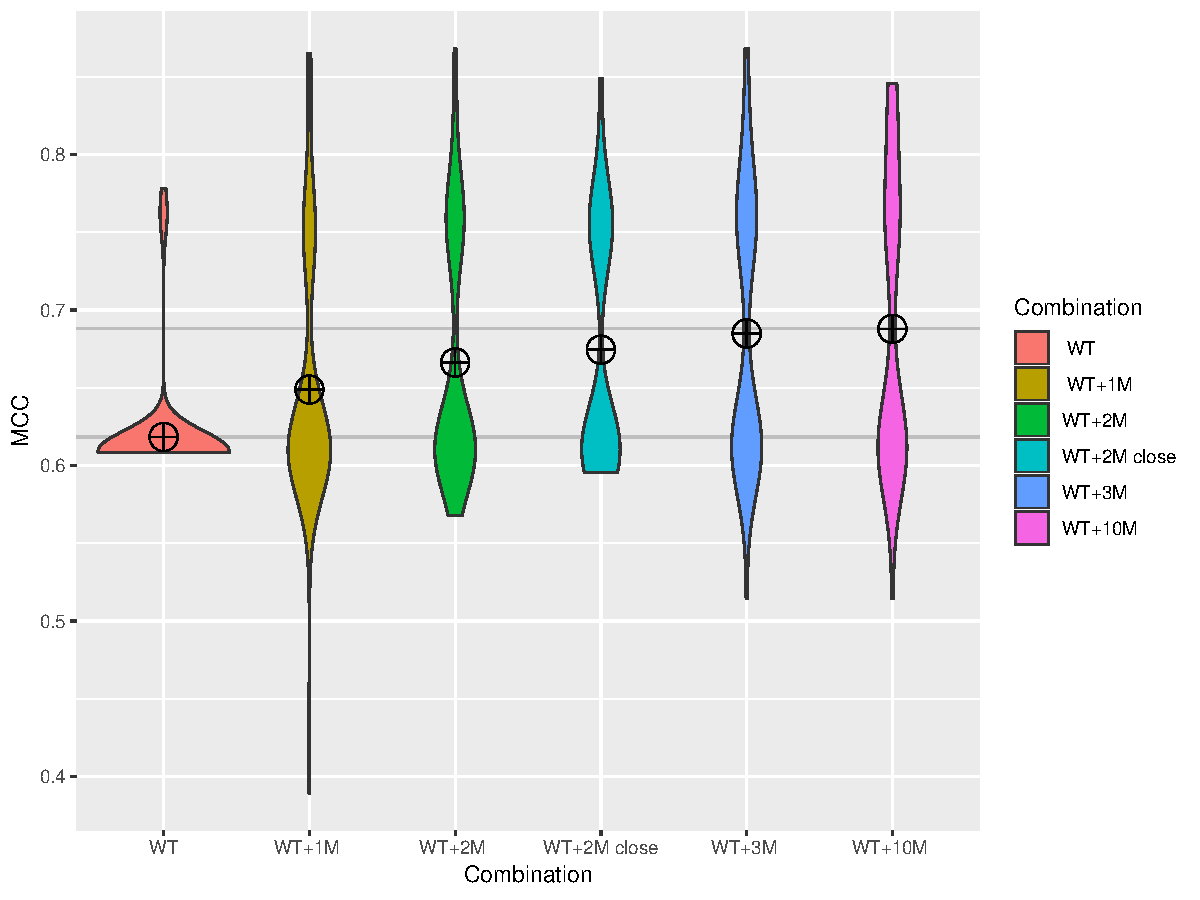
\includegraphics[width=\linewidth]{graphs/combinationscale}\\}
		
	\caption{Prediction accuracy (MCC) when considering the WT, supplemented with a set of $k=$1, 2, 3, or 10 single-point mutants, selected uniformly at random ({\sf WT+$k$M}). For 2 mutants, we also considered selecting mutants from the 20 most similar to the WT.}\label{fig:variantanalysis}
\end{figure}


%\begin{figure}[h]
%\begin{center}
%\includegraphics[scale=.4]{graphs/WT+combin}
%\label{Vsrsample}
%\caption{Accuracy of prediction reported as the MCC when considering only the WT, considering one mutants along side the WT and considering 10 mutants in addition to the WT.}

%\end{center}
%\end{figure}




%------------------------------------------------------------------------------

%======================




\section{Conclusion}

We introduce \OurTool{}, an integrative method for the prediction of secondary structure models from multiple probing profiles. Based on the simple premise that good structural models should be stable and supported by most probing experiments, it uses a combination of stochastic backtrack in the pseudo-Boltzmann ensemble, coupled with a structural clustering to elect dominant conformations. This strategy is fast, stable and leads to predictions that clearly benefit from the availability of multiple probing profiles, as demonstrated by a detailed analysis of three datasets. 


\OurTool currently represents the only available option for a joint automated consideration of multiple probing profiles.  Surprisingly, it also appears to outperform existing methods on single profiles on the Hadjin\etal\cite{Hajdin2013} dataset. We attribute this unexpected result to the adoption of a sampling/clustering approach, which appears able to eliminate spurious outliers in the conformational space. Indeed, while quite similar in its approach to Spasic et al, \OurTool seems to achieve better performance, calling for further analysis. 
Mainly, the adaptive choice of the number of clusters, even in cases where a single dominant conformation is expected, seems to create more opportunities for discarding random unstable conformations. Such conformations naturally occur in a Boltzmann-distributed subset of structures, and may end up \emph{polluting} centroid structures by artificially inflating the diversity within the cluster. The impact on \Software{RSample} predictions of such a \emph{noise} is  worsened by the fact that it returns the MEA, the centroid of the whole ensemble, whenever a dominant conformation is detected.

Our analyses reveal that integrating multiple profiles to at least three conditions allows to mitigate the effect of outlier conditions and, frequently, to produce better secondary structure models than the one inferred from the most accurate profile. A comparison of the joint performances to the average seems justified in a context where no single reagent appears to systematically dominate in term of predictive capacity, depriving the modeler from an objective way to favor a probing condition over another. Moreover, in realistic structure modeling scenarii, it is impossible to know \emph{a priori} which information is contributed by an experiment. In other words, combining experimental probing data, even in a pairwise fashion, typically mitigates the empirical risk of misprediction. 


Using probing conditions with our without Mg to use as constraints is a dilemma. In deed, RNA reach its native 3D structure mainly in the presence of Mg2+ ions (ref ). However, 3D includes non WC parings, and motifs such as pseudoknots, kissing loops, tetraloop interactions that RNA structure prediction algorithm do not take into account. In contrast in presence of monovalent but no divalent ions, RNA is suppose to adopt a structure in which all helical domains are formed but where most if not all tertiary contacts are not stable. Therefore one could assume that probing the RNA without Mg2+ provides signals that are more compatible and less deceptive for predicting algorithms. However it is likely that the instability of all the tertiary contacts is a situation prone to misfolding, or at least the coexistence in solution of many conformations. Here, the Dydimium ribozyme which contains many tertiary motifs was systematically probed in presence or absence of Mg2+ (except for CMCT and DMS). Remarkably, the best prediction were obtained with 1M7 and NMIA with our without Mg with very similar MCC, although the probing profile in the two conditions are quite divergent. For all the other reagents/protocols, prediction using constraints from experiments containing Mg2+ systematically outperform its counterpart without Mg2+ with a 0.1 average decrease of the MCC.
%\item je pense qu'il serait intéressant au moins pour un uo deux réactif de voir ce que donne le couple + et - Mg. Peut etre par exemple avec le 1M7ilu et un autre mauvais genre le NAI
%\end{itemize}
% il faudrait regrder ce que fait weeks avec le 1M7, le NMIA et le 1M6, je n'ai pas bien compris quelle tambouille il fait, mais ca part du meme genre de constatation : il y a une spécificité dans chacune des sondes qu'il n'arrive pas vraiment à formaliser donc il fait une tambouille qui lui permet de tous les intégrer (mais c'est peut etre un peu pédestre comme démarche!). Apres ce sont probablement des conditions tres proches ce qui n'apporte pas d'apres nos résultats bcq d'infos supplémentaires .. bref ca vaudrait peut etre le coup de comparer.


\paragraph{Reproducibility}

\paragraph{Pseudo-potentials}


\begin{figure*}
	{\centering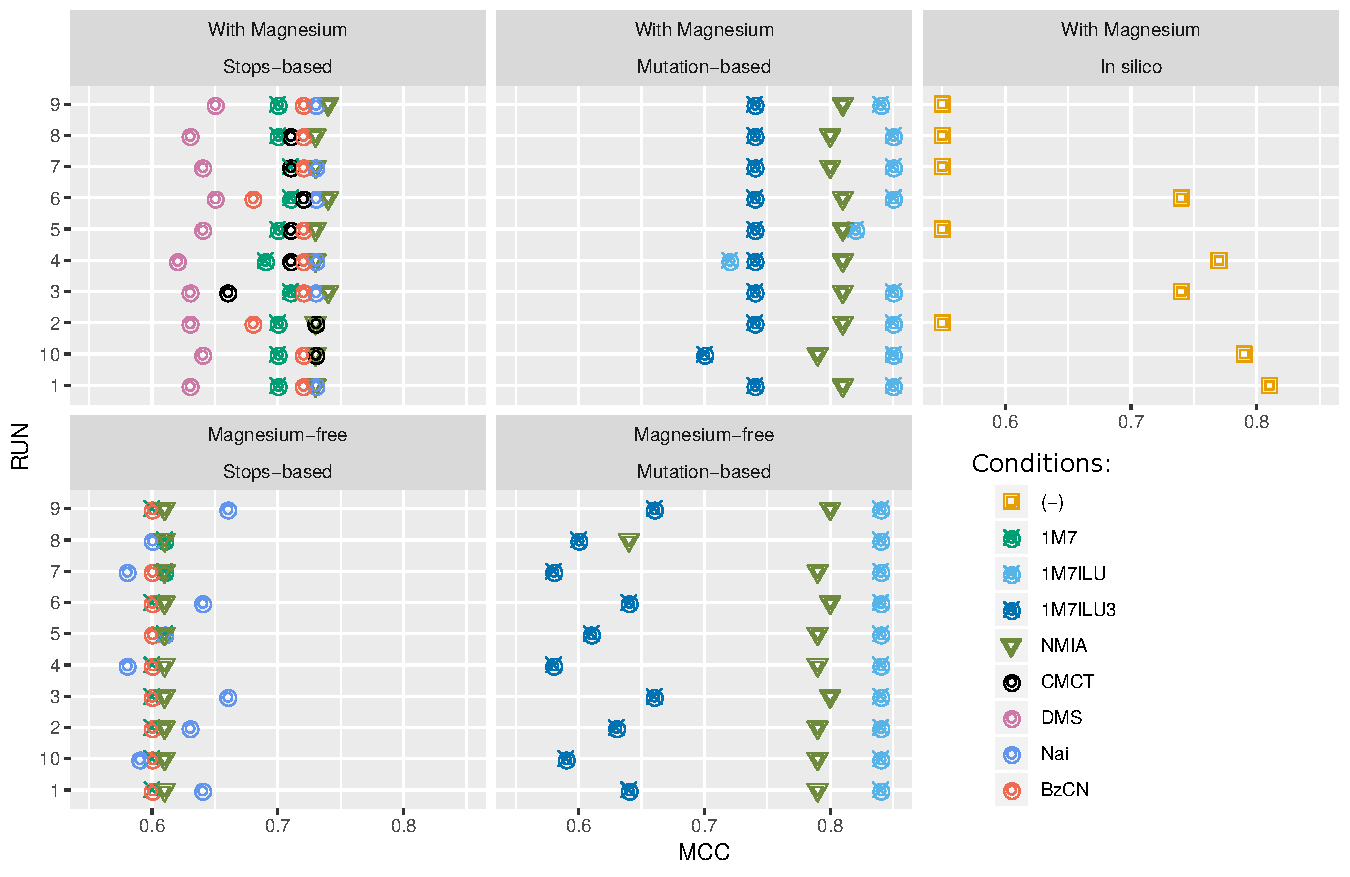
\includegraphics[width=1\linewidth]{graphs/Reproductibility}\\}
	
	\caption{MCC of predicted structures under conditions with and without Mg$^{2+}$, differentiating stop-inducing and mutation-inducing protocols, over 10 runs of IPANEMAP. }\label{fig:reproducibility}
\end{figure*}




%
%%discussion et conclusion sont fusionnés dans ce type d'article.}
%
%
%
%\begin{itemize}
%	\item Our integrative approach compared to other tools did exhibit a trade-off  between  number of optimal clusters and accuracy but remains fast to execute. 
%	\item While based on the assumption that the different probing condition reveal complementary aspects of the same structure, it can still be enriched by experiments where the dominant conformation is expected to differ from the native one.
%	
%	\item 
%	
%	\item Complementarity
%	\item Pseudo-Energy models
%\end{itemize}


\section*{Acknowledgements}
The authors wish to thank Ronny Lorenz for developing a probing-informed version of RNAsubopt, allowing to sample the pseudo-Boltzmann ensemble, and Nathalie Chamond for helpful suggestions.

\section*{Funding}
This work has been supported by La Fondation pour la Recherche Medicale ([FRM
DBI20141423337]).
%\bibliographystyle{bioinformatics}
\bibliographystyle{nar}
%\bibliographystyle{natbib}%compa
\bibliography{biblio}

\end{document}
